\documentclass[titlepage,openright,twoside,a4paper,10pt]{report}

\usepackage[top=3.5cm, left=3cm, right=3cm, bottom=2.5cm]{geometry}
\usepackage[unicode]{hyperref}
\usepackage{siunitx}
\usepackage{wrapfig}
\usepackage{footnote}
\usepackage[version=4]{mhchem}
\usepackage{enumitem}
\usepackage{graphicx}
\usepackage{fancyhdr}

% Approved Packages Above

\usepackage{csquotes}
\usepackage{titlesec}
\usepackage{titletoc}

% Not sure if I am using these above

\usepackage[table,xcdraw]{xcolor} %Used to color parts of tables for highlighting.
\usepackage[export]{adjustbox}
\usepackage{tikz} % For drawing detailed shapes etc.
\usepackage{float} % Defining new categories like figure, algorithm etc. and placing them however you want.
\usepackage{multicol} % For text or math in two columns, like in some papers.
\usepackage{cleveref} % For referencing anything without a specific type, it detects the type on its own.

% Useful but not used above

% Languages and Text Fonts
\usepackage[font={small}, labelfont=bf]{caption}
\usepackage{subcaption}
\usepackage{fontspec}
\usepackage{polyglossia}
\setdefaultlanguage{english}
\setotherlanguage[variant=modern]{greek}
\setmainfont{GFS Didot}

% Glossary and Acronyms
\usepackage[toc,nonumberlist,nopostdot,acronyms,automake]{glossaries}
\setglossarystyle{long}
% References
\usepackage[backend=biber,style=ieee]{biblatex}
% PDF Navigation Bookmarks
\usepackage{bookmark}

% Maths packages
\usepackage{amsmath, amssymb}
\usepackage{mathtools}
\usepackage{nicefrac}

\raggedbottom % Prevent huge spaces from the twoside option

% My Commands
\newcommand{\paper}[2]{#1 et al. \cite{#2}} % Citation reference function.
\newcommand{\mytitle}{Decoding and Classification of Category-Specific Visual Stimuli in the Fusiform Face Area Using fMRI Data and Machine Learning} % Command for easily typing my title.
\newcommand{\draft}[1]{{\leavevmode\color{red!90!black}#1}} % Highlight draft text areas, for revision and corrections.

% PDF properties
\definecolor{dark_grey}{HTML}{303030} % Colors

\hypersetup{
  pdfstartview= {FitH},
  pdfauthor   = {Nikolaos Kasapakis},
  pdftitle    = {\mytitle},
  pdfsubject  = {Bachelor thesis at the Department of Physics of the Aristotle University of Thessaloniki},
  pdfkeywords = {Neuroscience},
  colorlinks  = true,		%Colours links instead of ugly boxes
  urlcolor    = blue,		%Colour for external hyperlinks
  linkcolor   = dark_grey,		%Colour of internal links
  citecolor   = blue,		%Colour of citations
  bookmarksnumbered,
}

\addbibresource{references.bib}

\makeglossaries
\newacronym{MVPA}{MVPA}{Multi-Variate Pattern Analysis}
\newacronym{UPA}{UPA}{Univariate Pattern Analysis}
\newacronym{SVM}{SVM}{Support Vector Machine}
\newacronym{ROI}{ROI}{Region of Interest}
\newacronym{ROIs}{ROIs}{Regions of Interest}
\newacronym{BOLD}{BOLD}{Blood-Oxygen-Level-Dependent}
\newacronym{HbR}{HbR}{deoxyhemoglobin}
\newacronym{HbT}{HbT}{total hemoglobin}
\newacronym{HbO}{HbO}{Oxyhemoglobin}
\newacronym{Hb}{Hb}{hemoglobin}
\newacronym{OEF}{OEF}{Oxygen Extraction Fraction}
\newacronym{HCP}{HCP}{Human Connectome Project}
\newacronym{WM}{WM}{Working Memory}
\newacronym{ITI}{ITI}{inter-task interval}
\newacronym{CSF}{CSF}{Cerebrospinal Fluid}
\newacronym{RF}{RF}{radio frequency}
\newacronym{CBF}{CBF}{Cerebral Blood Flow}
\newacronym{ASL}{ASL}{Arterial Spin Labeling}
\newacronym{USA}{USA}{United States of America}
\newacronym{T1w}{T1w}{T1-weighted}
\newacronym{T2w}{T2w}{T2-weighted}
\newacronym{MZ}{MZ}{monozygotic}
\newacronym{DZ}{DZ}{dizygotic}
\newacronym{IQ}{IQ}{intelligence quotient}
\newacronym{T-MEG}{T-MEG}{task-evoked MEG}
\newacronym{EV}{EV}{explanatory variable}
\newacronym{COPE}{COPE}{contrast of parameter estimates}
\newacronym{SVMs}{SVMs}{Support Vector Machines}
\newacronym{PCA}{PCA}{Principal Component Analysis}
\newacronym{ICA}{ICA}{Independent Component Analysis}
\newacronym{PDF}{PDF}{probability density function}
\newacronym{HRF}{HRF}{Hemodynamic Response Function}
\newacronym{GLM}{GLM}{General Linear Model}
\newacronym{NIfTI}{NIfTI}{Neuroimaging Informatics Technology Initiative}
\newacronym{LR}{LR}{Left to Right}
\newacronym{RL}{RL}{Right to Left}
\newacronym{FEAT}{FEAT}{FMRIB's Expert Analysis Tool}
\newacronym{3D MPRAGE}{3D MPRAGE}{three-dimensional magnetization-prepared rapid gradient-echo imaging}
\newacronym{FOV}{FOV}{Field of View}
\newacronym{BW}{BW}{Bandwidth}
\newacronym{ES}{ES}{Echo Spacing}
\newacronym{BCI}{BCI}{Brain-Computer Interface}

% fMRI Acronyms
\newacronym{r-fMRI}{r-fMRI}{resting-state fMRI}
\newacronym{t-fMRI}{t-fMRI}{task-evoked fMRI}
\newacronym{dMRI}{dMRI}{diffusion imaging}
\newacronym{fMRI}{fMRI}{Functional Magnetic Resonance Imaging}
\newacronym{MRI}{MRI}{Magnetic Resonance Imaging}
\newacronym{MR}{MR}{Magnetic Resonance}
\newacronym{NMR}{NMR}{Nuclear Magnetic Resonance}

% Imaging Techniques Acronyms
\newacronym{PET}{PET}{Positron Emission Tomography}
\newacronym{NIRS}{NIRS}{Near Infrared Spectroscopy}
\newacronym{MEG}{MEG}{Magnetoencephalogram}
\newacronym{EEG}{EEG}{Electroencephalography}

% Brain Anatomy Acronyms
\newacronym{LGN}{LGN}{Lateral Geniculate Nucleus}
\newacronym{MT}{MT}{Middle Temporal visual area}
\newacronym{IT}{IT}{Inferior Temporal cortex}
\newacronym{FFA}{FFA}{Fusiform Face Area}
\newacronym{PPA}{PPA}{Parahippocampal Place Area}
\newacronym{LOC}{LOC}{Lateral Occipital Cortex}
\newacronym{EBA}{EBA}{Extrastriate Body Area}
\newacronym{FBA}{FBA}{Fusiform Body Area}
\newacronym{FG}{FG}{Fusiform Gyrus}
\newacronym{fSTS}{fSTS}{Superior Temporal Sulcus}
\newacronym{OFA}{OFA}{Occipital Face Area}
\newacronym{MOG}{MOG}{Middle Occipital Gyrus}
\newacronym{IOG}{IOG}{Inferior Occipital Gyrus}
\newacronym{LOS}{LOS}{Lateral Occipital Sulcus}

% Establishments Acronyms
\newacronym{WashU}{WashU}{Washington University}
\newacronym{UMinn}{UMinn}{University of Minnesota}
\newacronym{SLU}{SLU}{Saint Louis University}
\newacronym{NIH}{NIH}{National Institutes of Health}

% Glossary Entries
\newglossaryentry{V1}
{
	name = {V1},
	description = {Visual area V1, the striate cortex or primary visual cortex.\newline}
}

\newglossaryentry{V2}
{
	name = {V2},
	description = {Visual area V2, or secondary visual cortex, also called prestriate cortex.\newline}
}

\newglossaryentry{V3}
{
	name = {V3},
	description = {Visual area V3, which communicates directly with the respective dorsal and ventral subsystems of V2. It is less well-defined compared to other areas of the visual cortex.\newline}
}

\newglossaryentry{V4}
{
	name = {V4},
	description = {Visual area V4, a mid-tier cortical area in the ventral visual pathway.\newline}
}

\newglossaryentry{blob cells}
{
	name = {blob cells},
	description = {V1 cells that resemble kLGN neurons. They are monocular, color sensitive, characterized by small, concentric receptive fields and are found in clusters, hence the name.\newline}
}

\newglossaryentry{interblob cells}
{
	name = {interblob cells},
	description = {V1 cells, the majority of which are binocular, not color sensitive, characterized by elongated receptive fields, exhibit ocular dominance and orientation specificity, while they are found around the clusters of V1 blob cells.\newline}
}

\newglossaryentry{gyromagnetic ratio}
{
	name = {gyromagnetic ratio},
	description = {The gyromagnetic ratio, a constant specific to each different nucleus.\newline}
}

\newglossaryentry{TE}
{
	name = {Time of Echo},
	description = {The time between the delivery of the RF pulse and the receipt of the echo signal.\newline}
}

\newglossaryentry{TR}
{
	name = {TR},
	description = {The amount of time that passes between consecutive acquired brain volumes.\newline}
}

\newglossaryentry{flip angle}
{
	name = {flip angle},
	description = {The amount or rotation that net magnetization experiences during application of a RF pulse.\newline}
}

\newglossaryentry{connectomics}
{
	name = {connectomics},
	description = {The production and study of connectomes: comprehensive maps of connections within an organism's nervous system.\newline}
}

\newglossaryentry{2C}
{
	name = {2C},
	description = {The FEAT analysis that produced 2 chunks per subject, with a total of 40 chunks.\newline}
}

\newglossaryentry{4C}
{
	name = {4C},
	description = {The FEAT analysis that produced 4 chunks per subject, with a total of 80 chunks.\newline}
}

\pagenumbering{roman}

% Section Depth, ToC format, paragraph format.
\setcounter{secnumdepth}{4}
\setcounter{tocdepth}{4}
\titleformat{\paragraph} [hang] {\normalfont\normalsize\bfseries} {\theparagraph} {1em} {}

%%%%% End of Package Operations %%%%%

%% Intentionally left blank message
% https://gist.github.com/philipptempel/5220000
\makeatletter % Treats the @ symbol as a plain letter.
    \def\cleardoublepage{\clearpage%
        \if@twoside
            \ifodd\c@page\else
                \vspace*{\fill}
                \hfill
                \begin{center}
                This page intentionally left blank.
                \end{center}
                \vspace{\fill}
                \thispagestyle{empty}
                \newpage
                \if@twocolumn\hbox{}\newpage\fi
            \fi
        \fi
    }
\makeatother % Treats the @ symbol normally again.
%% End Intentionally left blank message

%% Start Fancy header settings
\pagestyle{fancy}
\fancyhf{}		% Clear all pre-set header and footer settings.
% Add the page number on the header in plain style pages. Works well for two - sided documents.
\fancypagestyle{plain}{
  \fancyhf{}
  \renewcommand{\headrulewidth}{0pt}
  \fancyhf[LEH,ROH]{\thepage}
}

% RE: right header of even pages.
% LO: Left header of odd pages.
\fancyhead[RE]{\itshape\nouppercase{\leftmark}}
\fancyhead[LO]{\itshape\nouppercase{\rightmark}}
\fancyhead[LE,RO]{\thepage}
%% End Fancy header settings

\begin{document}

\begin{titlepage}
\begin{figure}[H]
    \centering
    
\includegraphics[width=5cm]{assets/logo/AUTh_Logo.pdf}
    \label{fig:cover_auth_logo}
\end{figure}

\centering
\Large \href{https://www.auth.gr/}{\textbf{Aristotle University of Thessaloniki}}\\
\large \href{http://www.sci.auth.gr/}{Faculty of Sciences}\\
\large \href{https://www.physics.auth.gr/}{Department of Physics}

\vspace{18pt}

\large Bachelor Thesis
\vspace{12pt}

\begin{minipage}[t]{0.5\textwidth}
    \raggedright
    \begin{tabular}{ll}
        \textit{\textbf{Author:}} & \\
        \href{https://github.com/kasapakis-nk}{Kasapakis Nikolaos}\footnotemark[1] & \\
        %  & 
    \end{tabular}
\end{minipage}
\begin{minipage}[t]{0.49\textwidth}
    \raggedleft
    \begin{tabular}{rr}
        \textit{\textbf{Supervisor:}} & \\
        \href{https://www.physics.auth.gr/people/129}{Prof. Theodoros Samaras}\footnotemark[2] & \\
        %  & 
    \end{tabular}
\end{minipage}

\footnotetext[1]{\href{mailto:nkasapak@auth.gr}{nkasapak@auth.gr},  \href{https://github.com/kasapakis-nk}{\textit{https://github.com/kasapakis-nk}}}
\footnotetext[2]{\href{mailto:theosama@auth.gr}{theosama@auth.gr}, \href{https://www.physics.auth.gr/people/129}{\textit{https://www.physics.auth.gr/people/129}}}

\noindent\makebox[\linewidth]{\rule{\textwidth}{0.5pt}}\\[0.2cm]
\LARGE{\textbf{Decoding and Classification of Category-Specific Visual Stimuli in the Fusiform Gyrus Using fMRI Data and Machine Learning}}
\noindent\makebox[\linewidth]{\rule{\textwidth}{0.5pt}}\vspace{0.2cm}
\vspace{2pt}
%\vspace{8pt} % For 2 line title.
\large\today

\begin{figure}[H]
    \centering
    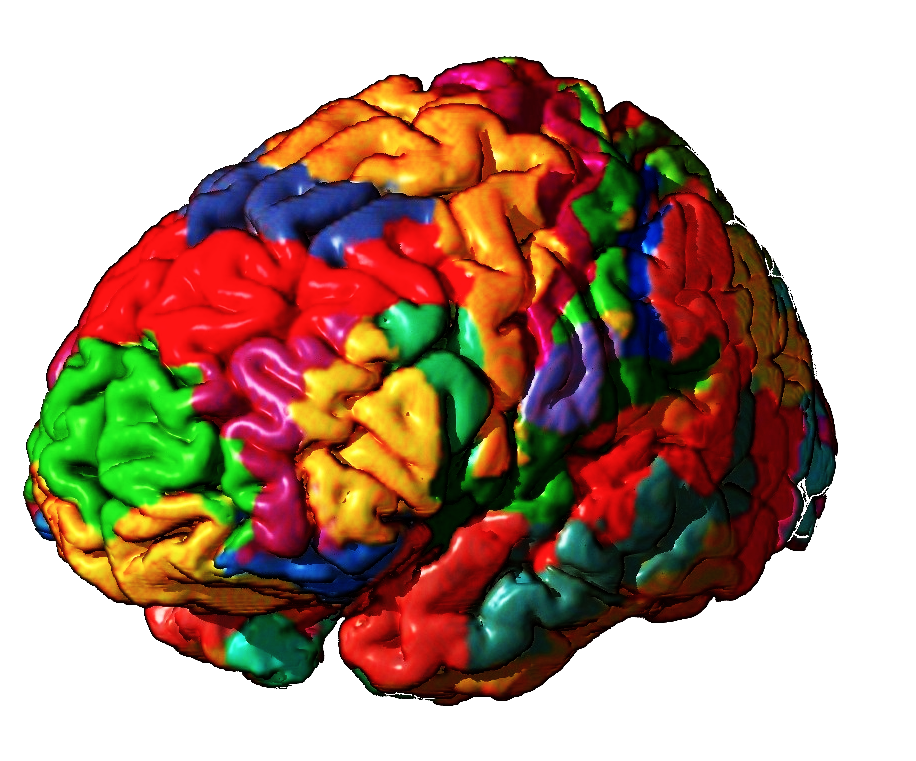
\includegraphics[height=7cm]{assets/images/brain_segmentation.png}
    \label{fig:brain_segmentation}
\end{figure}
%\vspace{-10pt} % For 2 line title.
\vspace{-16pt}

\vspace*{\fill}
\begin{minipage}[t]{0.5\textwidth}
\begin{figure}[H]
    
\includegraphics[width=4cm,left]{assets/logo/PhysicsLogo_English.pdf}
\end{figure}
\end{minipage}
\begin{minipage}[t]{0.49\textwidth}
\begin{figure}[H]
    
\includegraphics[width=2cm,right]{assets/license/by-sa.png}
\end{figure}
\end{minipage}
\footnotetext[3]{This thesis is licensed under the \href{https://creativecommons.org/licenses/by-sa/4.0/}{Creative Commons Attribution-Sharealike 4.0 Int. License (CC BY-SA 4.0).}}

\end{titlepage}


%\maketitle

\cleardoublepage
\thispagestyle{plain}
\vspace*{\fill}
\begin{center}
    \LARGE
    \textit{\textbf{Abstract}}
        
    \vspace{0.4cm}
    \large
    \textbf{Decoding and Classification of Category-Specific Visual Stimuli in the Fusiform Gyrus Area Using fMRI Data and Machine Learning}
        
    \vspace{0.4cm}
    Kasapakis Nikolaos
\end{center}
\normalsize

\vspace{0.9cm}

This thesis examines the use of \gls{fMRI} data from the \gls{HCP} to analyze neural systems involved in the processing of category-specific visual stimuli. It focuses on the \gls{WM} task within a broad \gls{fMRI} paradigm designed to explore various neural domains including visual, language, and decision-making systems. Specifically, the study examines brain activation patterns in the \gls{FG} related to different stimulus categories such as faces, places, tools, and body parts. Employing a pipeline of preprocessing steps followed by \gls{MVPA}, the research assesses distributed patterns of voxel activation allowing for complex and detailed analyses of cognitive states. Data is processed through a \gls{SVM} classification script developed for this study, aiming to differentiate between faces and other stimulus categories based solely on \gls{fMRI} data. The thesis also addresses classification methodologies, with a particular focus on optimizing classifier accuracy by adjusting parameters like the number of data chunks, fold counts for cross-validation, and subject counts. The findings offer insights into the distinct brain activation patterns associated with different stimuli in the \gls{FG}, contributing to our understanding of neural mechanisms in cognitive processes and practical applications for these insights.

\vspace*{\fill}

%\footnote{Temporal refers to time-related when used in the context of electromagnetics.}
%Creates a footnote in the same page with that message.

\cleardoublepage
\thispagestyle{plain}
\vspace*{\fill}
\begin{center}
    \LARGE
    \textit{\textbf{Περίληψη}}
        
    \vspace{0.4cm}
    \large
    \textbf{Αποκωδικοποίηση και Κατηγοριοποίηση Κατηγορικών Οπτικών Ερεθισμάτων στην Ατρακτοειδή Έλικα με Χρήση Δεδομένων fMRI και Μηχανικής Μάθησης}
        
    \vspace{0.4cm}
    Κασαπάκης Νικόλαος
\end{center}
\normalsize

\vspace{0.9cm}

Αυτή η εργασία εξετάζει τη χρήση δεδομένων λειτουργικής μαγνητικής τομογραφίας (\acrshort{fMRI}) από το \acrshort{HCP} για την ανάλυση των νευρωνικών συστημάτων που εμπλέκονται στην επεξεργασία κατηγορικών οπτικών ερεθισμάτων. Επικεντρώνεται στη δοκιμασία Λειτουργικής Μνήμης (\acrshort{WM}) μέσα σε ένα ευρύτερο πείραμα fMRI που έχει σχεδιαστεί για να εξερευνήσει διάφορους νευρωνικούς τομείς, συμπεριλαμβανομένων των συστημάτων όρασης, γλώσσας και λήψης αποφάσεων. Συγκεκριμένα, η μελέτη εξετάζει τα μοτίβα ενεργοποίησης του εγκεφάλου στην περιοχή της Ατρακτοειδούς Έλικας που σχετίζονται με διάφορες κατηγορίες οπτικών ερεθισμάτων, όπως πρόσωπα, τοποθεσίες, εργαλεία και μέρη του σώματος. Χρησιμοποιώντας μια σειρά προεπεξεργαστικών βημάτων ακολουθούμενη από Ανάλυση Πολυδιάστατων Μοτίβων (\acrshort{MVPA}), η έρευνα αξιολογεί κατανεμημένα μοτίβα ενεργοποίησης, επιτρέποντας σύνθετες και λεπτομερείς αναλύσεις των γνωστικών καταστάσεων. Τα δεδομένα επεξεργάζονται μέσω ενός υπολογιστικού προγράμματος κατηγοριοποίησης \acrshort{SVM} που αναπτύχθηκε για αυτή τη μελέτη, με στόχο τη διάκριση μεταξύ προσώπων και άλλων κατηγοριών ερεθισμάτων βασισμένων αποκλειστικά σε δεδομένα \acrshort{fMRI}. Η εργασία εξετάζει επίσης μεθοδολογίες ταξινόμησης, δίνο\-ντας ιδιαίτερη έμφαση στη βελτιστοποίηση της ακρίβειας του κατηγοριοποιητή με την προσα\-ρμογή παραμέτρων όπως ο αριθμός των ανεξάρτητων τμημάτων δεδομένων, ο αριθμός επανα\-ληπτικών διασταυρώσεων για επικύρωση και ο αριθμός των υποκειμένων των οποίων τα δεδομένα εμπλέκονται. Τα ευρήματα προσφέρουν πληροφορίες για τα διακριτά μοτίβα ενεργο\-ποίησης του εγκεφάλου που σχετίζονται με διάφορα ερεθίσματα στην Ατρακτοειδή Έλικα, συμβάλλοντας στην κατανόησή μας για τους νευρωνικούς μηχανισμούς στις γνωστικές διαδικα\-σίες και στην ανάπτυξη πιθανών πρακτικών εφαρμογών μέσω αυτών των ευρημάτων.

\vspace*{\fill}



\cleardoublepage
\thispagestyle{plain}
\begin{center}
    \LARGE
    \textit{\textbf{Acknowledgements}}
        
    \vspace{0.4cm}
\end{center}
\normalsize

\vspace{0.9cm}

First and foremost, I would like to express my deepest gratitude to Professor Theodoros Samaras for his support and guidance throughout every stage of this work. I am equally indebted to PhD candidate Dimitris Stoupis, whose expertise in academic matters, neuroscience, neuroanatomy, coding and statistics was instrumental in navigating the complexities of this research. His constant assistance and acumen were crucial to the successful completion of this project.

Beyond the technical work and analysis, the review process is crucial to ensuring the highest quality outcome. For this, I am profoundly grateful to my significant other, Ioanna-Anastasia Koukouli, for her unwavering support and encouragement throughout this journey. Her key insights into the design of this thesis were instrumental in shaping the final work, and her thoughtful input greatly enriched the overall direction of the project.

In any research endeavor, there are often unsung heroes who play a vital role behind the scenes. I believe it is essential to acknowledge them here. The open knowledge and open-source communities deserve special recognition for their immediate and high-quality support, whether through forums or mailing lists. Their collective wisdom greatly aided in resolving various technical challenges. I hope all contributors have been given the deserved credit.

\vspace*{\fill}



\pdfbookmark[1]{Table of Contents}{toc}
\tableofcontents

\listoffigures
\listoftables
\cleardoublepage

% Add the sections
\pagebreak
\pagenumbering{arabic}
\chapter{Theoretical Background}

\section{Introduction}

The significance of the sense of vision for humans, in our contemporary everyday lives as well as in our evolution as a species, cannot be understated. While there is no clear consensus that vision is our most important sense, since that is dependent on one's cultural, societal and technological influences, there exists a large body of data drawn from cross-sectional observational research and surveys, as well as expert opinion of practitioners and researchers that leans towards the fact that vision is considered the most valued sense to the public.

Since prehistoric times, it is our vision that has aided us in our survival, by means of allowing us to advantageously select healthy mates, forage ripe fruit against a green foliage and detect predators through their natural camouflage, just to name a few benefits. Even in today's world, the majority of the information we process hails from our eyesight, whether it originates from the environment or from a computer screen.

However controversial the topic of the superiority of vision over our other senses might be, what is truly undebatable is that our evolution and eventual dominance as a species has been a consequence of the capabilities of our brain. It is the current form of the human brain after all, displaying an astonishingly intricate way in which it processes visual stimuli, that was preferentially chosen through natural selection to translate visual information to fit the species' best interests. Thus, it could be argued that to achieve a holistic understanding of the sense of vision, we need to delve into the patterns of activation induced in the brain by visual stimulation.

\section{Visual Information Flow In The Brain}

Light entering the eye creates a cascade of neuronal events throughout the optic pathway, which describes the anatomical pathway by which electrical signals generated by the retina are sent to the brain.

\subsection{The Optic Pathway}

The optic pathway begins in the retina, which is a complex structure made up of ten different layers. Notably, the photoreceptor layers consist of the rods and cones, which generate action potentials with the help of rhodopsin through photosensitive cycles. The ganglion cell layer and nerve fiber layer serve as the foundation of the optic nerve; the former contains the cell bodies, and the latter contains the axons as they stream across the retina. The nerve is surrounded by the dura, which is a continuation of that of the brain, allowing free movement of \gls{CSF} between the eye and the intracranial vault. The axons exit the orbital part of the optic nerve through the orbital foramen, simultaneously with the ophthalmic artery and sympathetic fibers.

\clearpage

\begin{wrapfigure}{l}{0.42\textwidth}
	\centering
	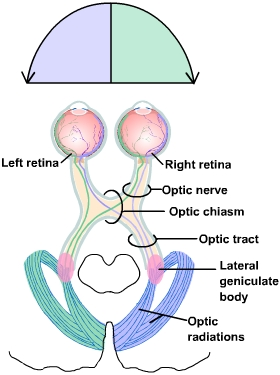
\includegraphics[width = 0.42\textwidth]{assets/images/Optic_Pathway.jpg}
	\caption[The Visual Pathway]{Illustation of the Visual Pathway and its components, including the course of information flow from the right (green) and left (blue) hemifields of the two eyes' visual fields. Adapted from \cite{optic_nerve}.}
	\label{fig:OpticPath}
\end{wrapfigure}

They then enter the optic canal, a bone-encased tunnel intended to protect the nerve, exit into the middle cranial fossa to form the intracranial part of the optic nerve, which continues till the two optic nerves join together to form the optic chiasm directly behind and above the pituitary stalk. Beyond the chiasm, the pathway continues as two distinct tracts, each carrying the temporal fibers from the other eye. The optic tract then passes posteriorly where most of the axons synapse in the layers of the \gls{LGN} of the midbrain, which is a posterolateral extension of the thalamus.

The majority of the fibers pass posteriorly to become the genico-calcarine tracts, which have both parietal and temporal loops and terminate into the cuneus gyrus and lingual gyrus of the primary visual cortex, respectively (see \autoref{fig:OpticPath}). Perception of sight ultimately derives from processing within this and adjacent areas of the brain \cite{Gupta2022}.

\subsection{Information Processing In The Visual Cortex}

\begin{wrapfigure}{l}{0.29\textwidth}
	\centering
	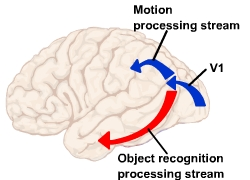
\includegraphics[width = 0.29\textwidth]{assets/images/Info_distinction_from_vis_cortex.jpg}
	\caption[Visual Information Flow Bifurcation]{Distinction in the flow of visual information from the \gls{V1} to other cortical areas. The ventral stream transfers information to the inferior cortical areas, whereas the dorsal stream tranfers it to the more superior cortex. Adapted from \cite{optic_nerve}. }
	\label{fig:processing_streams}
\end{wrapfigure}

The modules that compose the visual pathway from the retina to higher visual centers follow two diverging streams in the cortex: one pathway extends dorsally to terminate within the parietal lobe, including the motion detection area, \gls{MT}, and the visual areas of the posterior parietal cortex; the other pathway extends ventrally to terminate in the temporal lobe, including \gls{V4} and \gls{IT}. It is suggested \cite{Mishkin1983} that these two pathways serve different functions: the dorsal pathway is concerned with \textit{where} an object is in visual space (motion, distance); the ventral pathway is concerned with \textit{what} an object is (form, color, texture, all of which are involved in object recognition) (see \autoref{fig:processing_streams}).

The \gls{V1} area of the brain is involved in the initial cortical processing of all visual information necessary for visual perception. The color, shape and movement information from the thalamus are sent to different neurons within \gls{V1} for further processing and then sent onto different areas of the extrastriate visual cortex. 

Within \gls{V1}, information processed by \gls{blob cells} is used in color perception, color discrimination and the learning and memory of the color of objects. The \gls{blob cells} are the "color" processing cells of the \gls{V1}. On the other hand, \gls{V1} \gls{interblob cells} belong in one of two categories: The first are location specific cells, which respond best when the stimulus is in a specific location of the receptive field. The information processed by these cells is used in object perception, discrimination, learning and memory, or in spatial orientation. These cells are the "shape, form and location" cells of the \gls{V1}; The second kind of \gls{interblob cells} is the movement sensitive ones, which respond best to moving stimuli and are utilized to detect object movement, direction and velocity and to guide eye movements. These are the "motion detecting" cells of \gls{V1}.

The \gls{V1} sends input to the extrastriate visual cortex, which includes all the occipital lobe areas surrounding the \gls{V1}. The extrastriate cortex in non-human primates has been subdivided into as many as three functional areas, \gls{V2}, \gls{V3} and \gls{V4}. The information corresponding to each of the aforementioned categories of neurons in the \gls{V1} is sent  to different areas of the extrastriate visual cortex.

Specifically, the neurons in the inferior temporal visual association cortex, i.e., the ventrally located neurons accessed by the ventral stream, are responsible for processing information necessary for our abilities to recognize objects and colors, read text and learn and remember visual objects. It can thus be concluded that, in the context of this thesis, which investigates task-evoked visual stimulation, this area of the brain will be the region of interest. More deliberately, four regions of extrastriate cortex are of utmost importance for the purposes of this current dissertation: the \gls{FFA}, the \gls{PPA}, the \gls{LOC} and the \gls{EBA}.

\subsection{Category-Specific Information Processing Areas In The Extrastriate Visual Cortex}

% FFA Description
In the early 1990s, \gls{PET} demonstrated activation of the ventral visual pathway, especially the \gls{FG}, in a variety of face perception tasks \cite{Haxby1991, Sergent1992}. \gls{fMRI} studies of the specificity of these cortical regions for faces began with demonstrations of fusiform regions that responded more strongly to faces than to letter strings and textures \cite{Puce1996}, flowers \cite{McCarthy1997} and other mixed stimuli  \cite{Kanwisher1997}. Although face-specific \gls{fMRI} activations could also be seen in many subjects in the region of the \gls{fSTS} and in the occipital lobe in a region named the \gls{OFA}, the most consistent and robust face-selective activation was located on the lateral side of the mid-fusiform gyrus, within the \gls{IT}, in a region consequently named the \gls{FFA}. With the methods currently used, this region can be functionally identified in almost every normal subject in a short "localizer" \gls{fMRI} scan contrasting the response to faces versus objects \cite{Kanwisher2006}.

% PPA Description
Another well studied category-selective region of cortex is the \gls{PPA}, responding strongly to a wide variety of stimuli depicting places and/or scenes (e.g. outdoor and indoor scenes and houses) compared to various control stimuli such as faces or scrambled scenes \cite{Epstein1998}. Additionally, it has been found that \gls{PPA} activity is not affected by the subject's familiarity with the place depicted, does not increase when subjects experience a sense of motion through the scene, and is greater when viewing novel versus repeated images \cite{Epstein1999}. Using sets of scenes that had viewpoint changes, it was demonstrated that the \gls{PPA} treated scenes with viewpoint changes as different \cite{Epstein2003}, suggesting that this area represents scenes as individual snapshots of each view rather than as a broader scene that integrates multiple similar snapshots. However, when subjects saw different snapshot views from panoramic scenes, which represented clearly different views but appeared to come from the same scene, \gls{fMRI} showed no attenuation for panoramic repeats in the \gls{PPA}, suggesting viewpoint-specificity \cite{Park2009}.

% LOC Description
The \gls{LOC} is located on the lateral bank of the \gls{FG}, extending both ventrally and dorsally, consisting of the \gls{MOG} and the \gls{IOG} as well as the \gls{LOS} between them. This region has been shown to respond more strongly when subjects passively view photographs of common everyday objects than when they view visual textures without obvious shape interpretations \cite{Malach1995}. Importantly, the magnitude of the response was no different for familiar objects and unfamiliar ones with clear three-dimensional shape interpretations (e.g. Henry Moore sculptures). A similar result was found using line drawings \cite{Kanwisher1996}: stronger responses to three-dimensional objects depicted in line drawings, whether familiar or novel, compared to scrambled line drawings. Several more studies provide evidence that the entire \gls{LOC} region responds more strongly to intact objects with clear shape interpretations, than to control stimuli that do not depict clear shapes \cite{Kalanit1998, Murtha1999, Kalanit2001}.

% EBA Description
Since the turn of the twentieth century, neuroimaging studies have identified two brain regions of the extrastriate visual cortex that are highly sensitive to the perception of human bodies and body parts in comparison to other classes of stimuli. These regions are the \gls{EBA}, which is a body-selective focal region located partly at  both the posterior inferior temporal sulcus and the middle temporal gyrus \cite{Downing2001} and the \gls{FBA} found ventrally in the fusiform gyrus \cite{Peelen2005}. Evidence derived from \gls{fMRI} studies has shown that both areas become significantly activated in response to body and body parts stimuli visually presented in different formats such as photos, line drawings, stick figures and silhouettes compared to control stimuli like faces, tools and scenes \cite{Spiridon2006, Weiner2010, Amoruso2011}. Additionally, research seems to suggest that the \gls{EBA} also participates in more complex functions like body discrimination of self versus others. \cite{Pann2021}. It has been suggested that \gls{EBA} and \gls{FBA} can be functionally dissociated, with a more selective activation for local body parts in \gls{EBA} relative to more holistic images of the human body in \gls{FBA} \cite{Taylor2007}.

\begin{figure}[htbp]
 	\centering
	\begin{subfigure}{0.49\textwidth}
		\centering
		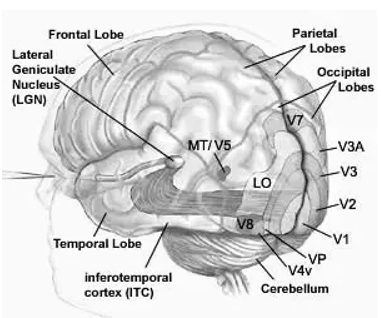
\includegraphics[width = 0.8\textwidth, height = 4cm]{assets/images/visual_areas.png}
		\caption{Graphic of the visual areas of the brain thought to be geographically within the occipital lobe \cite{visual_centers}. Adapted from \paper{Perez}{Perez2012}.}
		\label{fig:Visual_areas}
	\end{subfigure}
	\hfill
	\begin{subfigure}{0.49\textwidth}
		\centering
	 	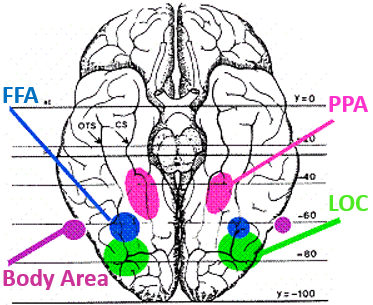
\includegraphics[width = 0.8\textwidth, height = 4cm]{assets/images/brain_areas.png}
		\caption{Brain diagram including some category-specific information processing areas of the brain \cite{prosopagnosia}. Adapted from \cite{brain_areas}.}
		\label{fig:Specific_areas}
	\end{subfigure}
	\caption[Brain Regions of Interest]{Illustration of \gls{ROIs} in the human brain.}
 	\label{fig:Brain_Areas}
\end{figure}

% Mutual exclusivity of category specific areas
While it has been clearly established that certain areas of the extrastriate visual cortex process category-specific information (see \autoref{fig:Brain_Areas}), another critical inquiry, particularly in the context of \gls{fMRI} \gls{MVPA} of contrasts among different classes of stimuli, is whether each region is exclusively selective for target-specific stimuli or if there is overlap between regions, especially considering the close proximity among them. One such case is the \gls{FFA} and \gls{FBA}, which have been found in many subjects to be adjacent or overlap with one another. However, in \gls{ROIs} that omit overlapping voxels it has been demonstrated \cite{Schwarzlose2005} that, \gls{FFA} showed no response above control objects for body stimuli and \gls{FBA} showed no response above control objects for face stimuli, confirming strong selectivities in distinct but adjacent regions in the \gls{FG}. Similar conclusions of high selectivity have been reached \cite{Mengjin2022} in regard to the \gls{FFA} and the \gls{PPA}, where results revealed distinct response properties between the two regions for faces and houses respectively, implying a combination of spatially discrete domain-specific and relatively distributed domain-general organization mapping in the human ventral temporal cortex.

% Neuroimaging techniques intro and segway into fMRI explanation
Many brain imaging tools are available to cognitive neuroscientists, including \gls{PET}, \gls{NIRS}, \gls{MEG}, \gls{EEG} and \gls{fMRI} \cite{Xue2010}. Some of those have had their time in the spotlight in the previous decades but have now been overshadowed by the more advanced, non-invasive neuroimaging techniques such as \gls{EEG} and \gls{fMRI}, which allow researchers to directly observe brain activities while subjects perform various perceptual, motor or cognitive tasks. It is therefore imperative that we acquire at least a basic understanding of the procedures and metrics through which these techniques work if we are to be able to interpret their results and further analyze them. For the purposes of this paper, we focus on the inner workings of \gls{fMRI}, which is the instrument used to extract the data used in our \gls{MVPA}.

\section{Mechanisms of Functional Magnetic Resonance Imaging}

\subsection{Fundamentals of NMR Signal Generation}

% Summary of NMR signal generation
The outline of the process by which \gls{fMRI} signal is generated begins with the scanner creating a powerful magnetic field  \( \vec{\boldsymbol{B_0}} \). All magnetic moments of nuclei with nonzero spin, including protons which are found overwhelmingly in the form of hydrogen nuclei in the human brain, tend to weakly align with \( \vec{B_0} \), creating a net macroscopic magnetization \( \vec{\boldsymbol{M_0}} \). A coil within the machine, then transmits a \gls{RF} transverse magnetic field at the resonant frequency \text{\( \omega_0 = \gamma \cdot B_0 \)}, where \( \boldsymbol{\gamma} \) is the \gls{gyromagnetic ratio}, tipping the magnetic moment from alignment and causing it to precess around the \( \vec{B_0} \) axis at angular frequency \( \boldsymbol{\omega_0} \). For protons, \text{\( \gamma = \ \SI{2.675e8}{\radian \per \tesla} \)} and at a typical magnetic field strength of \SI{3}{\tesla}, the precession frequency \text{\( \nu_0 = \omega_0 / 2\pi \)} is approximately \SI{128}{\mega\hertz}. Following this interaction, the net magnetization vector can be described as two components: the remaining longitudinal magnetization along the \( \vec{B_0} \) axis; and the rotating transverse magnetization perpendicular to \( \vec{B_0} \). The rotating component generates an oscillating magnetic field that induces a current in a nearby coil, thereby producing the basic measured \gls{NMR} signal. Over time, the transverse magnetization decays exponentially with a characteristic time constant \( \boldsymbol{T_2} \), and the longitudinal magnetization recovers exponentially towards its equilibrium value \( M_0 \) with a time constant \( \boldsymbol{T_1} \) \cite{Buxton2013, Suriaga2009}.

\subsection{Relaxation Time Constants}

% T1
T1 relaxation is the process by which the $z$ component of the net magnetization $M$ returns to its initial maximum value $M_0$ parallel to $B_0$. It can be modeled as a simple exponential with $T1$ as a first-order time constant, defining it as the time required for $M_z$ to reach $(1 - \frac{1}{e})$ or about $63\%$ of its maximum value (see \autoref{fig:T1} \cite{T1}). A typical value for $T1$, inside a \SI{3}{\tesla} magnetic field, in gray matter of the human brain is about $\SI{1.0}{\second}$. As $M_z$ grows toward $M_0$ the energy of the spin system decreases, considering that more spins statistically favor the spin-up parallel orientation, which is the lower of the two potential energy states. Consequently, as T1 relaxation occurs, energy dissipates from the system in the form of heat, hence the synonym for T1 relaxation, "thermal relaxation". This heat is then transferred to nearby nuclei via collisions, rotations, or electromagnetic interactions, and becomes unrecoverable. At its core, T1 relaxation represents an energy exchange process between spins and their external environment.

Blood inflow and \gls{CBF} can act to decrease the T1 values of blood and extravascular tissue components, resulting in a modified, measured T1 constant, termed T1*. Flowing blood moves spins from outside the imaging plane into the slice pixels. When spins in the imaging plane are saturated, signal from the unsaturated inflowing blood is enhanced relative to the surrounding stationary spins. The magnitude of this inflow contribution in vessels depends on the \gls{MRI} parameters, \gls{TR} and \gls{flip angle} $\theta$. When the \gls{TR} is sufficiently long to allow arterial blood spins from outside the imaging slice to flow into capillaries and exchange with extravascular tissue water, spatially specific perfusion contrast appears. In the extravascular tissue pool, \scalebox{1.2}{$\frac{1}{T_1^*} = \frac{1}{T_1} + \frac{f}{\lambda}$} where $f$ is the \gls{CBF} and $\lambda$ is the blood-to-tissue partition coefficient \cite{Detre1992}. 

\begin{figure}[htbp]
    \centering
    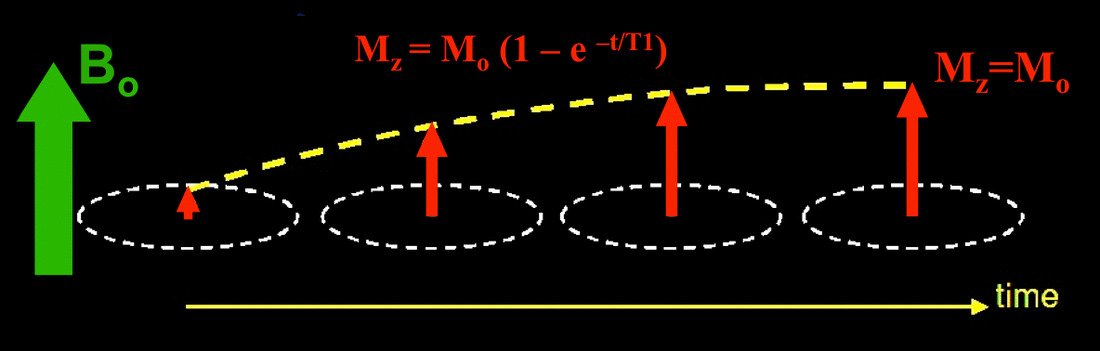
\includegraphics[width = 0.75\textwidth]{assets/images/T1_illustration.jpg}
    \caption[T1 Relaxation]{Illustration of T1 relaxation. Adapted from \cite{T1}.}
    \label{fig:T1}
\end{figure}

% T2
T2 is the time constant for decay or dephasing of transverse magnetization $M_{\text{xy}}$ and may occur with or without energy transfer. T2 relaxation is considered to follow first order kinetics, resulting in a simple exponential decay (identical to radioactive decay), resulting in T2 being the time required for the net transverse magnetization to fall to $\frac{1}{e}$ or approximately $37\%$ of its initial value \cite{T2}. Following a $90^\circ$ \gls{RF} pulse, the initial Boltzman distribution of spins in the $z$ direction, constituting $M_z$, is preserved and transformed by the rotation into what is termed "phase coherence" in the $\text{xy}$ plane, in the form of an asymmetrical clustering of spins which gives rise to a net transverse magnetization $M_{\text{xy}}$. After the pulse is over, the many transverse spin components will precess within the plane at the Larmor frequency. The presence of a non-zero $M_{\text{xy}}$ at any time, is evidence of persistent asymmetry of transverse components of angular momentum. Any process that disrupts either the number or the relative positions of said components will result in T2 relaxation. These fall into one of two general categories.

The first kind of T2 relaxation is when it accompanies T1 relaxation. If energy radiated during the latter, were to affect one of the spins contributing to $M_{\text{xy}}$, both its angular momentum components would be randomly changed, and it would immediately lose phase relations with other spins, thus it would stop contributing to $M_{\text{xy}}$ altogether. As a result, $M_{xy}$ would be diminished, meaning T2 relaxation would have occurred. We can conclude that any process causing T1 relaxation also results in T2 relaxation, while the opposite is not true. This is sometimes called the T1 contribution to T2 and explains why T1 needs to be monitored as well, even though it is the sweep of the transverse magnetization alone that induces a current in the receiver coils, ultimately producing the \gls{NMR} signal.

On the contrary, stand-alone T2 relaxation is referred to as the secular contribution to T2. One of the most common ways for this to occur is when a spin is situated in a molecular environment where it experiences a local static magnetic field disturbance \( B_{\text{loc}} \) in addition to \( B_0 \). The component \( B_{\text{loc}-z} \) of the secondary magnetic field, parallel to the main field, is added to the total magnetic field experienced by the spin, causing it to precess at a frequency \text{\( \omega_0^{\prime} = \gamma \cdot (B_0 + B_{\text{loc}-z}) \)}. Meanwhile, the unaffected spins continue to precess at the original Larmor frequency. Over time, a phase difference of \( \phi = \gamma \cdot B_{\text{loc}-z} \cdot t \) develops between the disturbed spin and the rest, leading to loss of phase coherence, T2 relaxation, and reduction in \( M_{\text{xy}} \). Secular T2 relaxation can also occur due to a special dipolar interaction, where a pair of spins simultaneously exchange their longitudinal angular momentum components, resulting in no net T1 effect but loss of T2 coherence. In gray matter in the human brain, at a field strength of 3 \si{\tesla}, measured T2 is around \( \SI{0.1}{\second} \).

\begin{figure}[htbp]
    \centering
    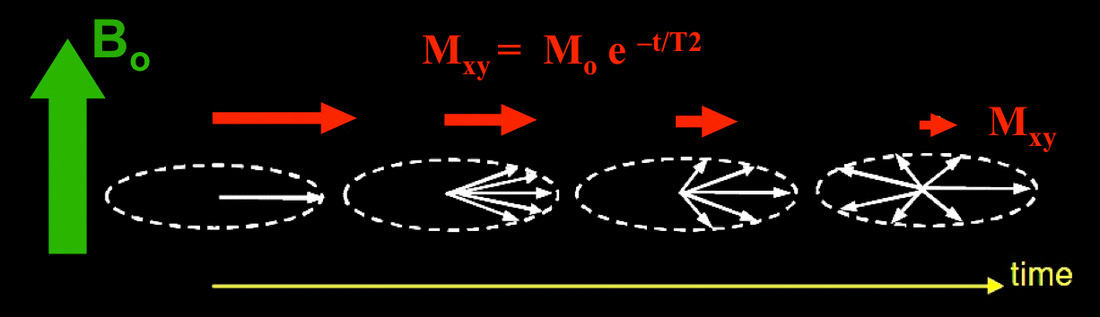
\includegraphics[width = 0.75\textwidth]{assets/images/T2_illustration.jpg}
    \caption[T2 Relaxation]{Illustration of T2 relaxation. Adapted from \cite{T2}.}
    \label{fig:T2}
\end{figure}

% T2*
It needs to be noted that in any real \gls{NMR} experiment, the transverse magnetization decays much faster than would be predicted by natural atomic and molecular mechanisms; this faster rate is denoted \textbf{T2*}. It can be considered as "observed" or "effective" T2, whereas the latter can be thought of as the natural T2 of the tissue being imaged. T2* is always less than or equal to T2 (see \autoref{fig:T2_star}). T2* results principally from inhomogeneities in the main magnetic field, which may arise from intrinsic defects in the magnet itself or susceptibility-induced field distortions caused by tissue or other materials within the field. Certain \gls{MR} sequences using gradient echoes and relatively long \gls{TE} values are called \gls{T2w} \cite{T2_star}.

% Mathematics of NMR signal
Pixel sizes in typical \gls{fMRI} studies are a few millimeters; each pixel may therefore include blood, extravascular tissue, and \gls{CSF}. Since arterial blood and venous blood have different T2 values, these should be considered separately, with the assumption that capillary content is partly arterial blood and partly venous blood. Thus, \gls{NMR} signal intensity from a pixel is the sum of signals originating from multiple compartments with different spin density and relaxation parameters. The \gls{fMRI} intensity $S$ can be described as seen in \autoref{eq:MRI_Signal_Intensity} \cite{Kim2012}.

\begin{equation}
	\label{eq:MRI_Signal_Intensity}
	S = \sum_i \rho_i \times V_i \times M_{\text{ss},i} \times e^{-\text{TE}/T_{2,i}^*}
\end{equation}

\begin{equation}
	\label{eq:ss_magnetization}
	\displaystyle M_{\text{ss},i} = \frac{\left(1 - e^{-\text{TR}/T_1^*}\right) \sin\theta}{1 - \cos\theta \times e^{-\text{TR}/T_1^*}}
\end{equation}

Subscripts \( i \) indicate each compartment; \( \rho \) is the water proton spin density, directly related to water content in the tissue; \( V \) is the volume fraction, which is approximately \( 1\% \) for arterial blood \cite{Ito2001} and \( 2.5 \text{-} 3\% \) for venous blood \cite{An2002a, An2002b}; \( M_{\text{ss}} \) is the steady-state magnetization given by \autoref{eq:ss_magnetization}; \( \textit{\gls{TR}} \) is the repetition time; \( T_1^* \) is the apparent longitudinal relaxation time in the presence of inflow; and \( \theta \) is the \gls{flip angle}. It should now be evident that \gls{fMRI} signal changes depend not only on imaging parameters, but also on biophysical responses that significantly affect these variables.

\begin{figure}[htbp]
    \centering
    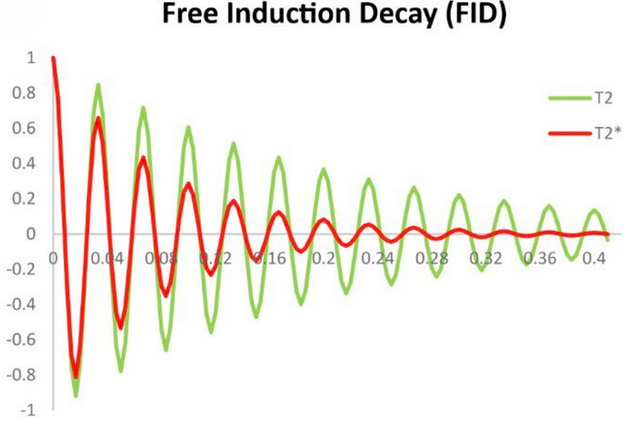
\includegraphics[width = 0.75\textwidth]{assets/images/FID.png}
    \caption[NMR Signal]{The observable \gls{NMR} signal generated by non-equilibrium nuclear spin magnetization precessing about $B_0$. Adapted from \cite{T2_star_graph}.}
    \label{fig:T2_star}
\end{figure}

% fMRI Techniques and segway into BOLD
At this point, with a solid grasp of the general physical quantities involved in the production of \gls{NMR} signals, it is important to link these quantities with biological processes in the human brain to progress from pure anatomical imaging to functional display. Several techniques can detect changes in metabolic activity following neural activation, including contrast \gls{fMRI}, \gls{BOLD} \gls{fMRI}, and perfusion \gls{fMRI}. Contrast \gls{fMRI} requires the injection of contrast agents such as iron oxide coated with sugar or starch. Although this method can provide relatively strong signals, researchers are often reluctant to use this semi-invasive method with healthy volunteers. Perfusion \gls{fMRI} utilizes \gls{ASL} to magnetically label hydrogen nuclei in arterial blood and then images their distribution in the brain. The signal received from this technique is more stable and less noisy than that of \gls{BOLD} \gls{fMRI}, but it is also relatively weak, and the length of image acquisition time makes it impractical for many applications. Currently, the most widely used \gls{fMRI} method is \gls{BOLD} imaging.

\subsection{Blood Oxygen Level Dependent \textit{(BOLD)} Signal}

% Short abstract of subsection.
The \gls{BOLD} signal, captured in \gls{fMRI} detects changes in \gls{HbR} driven by localized changes in brain blood flow and blood oxygenation, which are coupled to underlying neuronal activity by a process termed neurovascular coupling. \gls{fMRI} relies upon the measurement of T2* relaxation, which is sensitive primarily to local concentrations of paramagnetic \gls{HbR} in venous blood, rendering the latter a naturally occurring contrast agent. Interpretation of the \gls{fMRI} \gls{BOLD} signal is intrinsically linked to understanding the underlying physiological and metabolic processes in the brain that modulate blood flow.

% How BOLD manifests.
The \gls{BOLD} effect related to neural activity arises because of two distinct phenomena. The first is that when \gls{Hb}-the molecule in blood that carries oxygen-lose the oxygen to become \gls{HbR}, its magnetic properties change in a subtle way: \gls{HbR} is paramagnetic, and alters the magnetic susceptibility of blood, whereas \gls{HbO} and the surrounding tissue \ce{H2O} are diamagnetic (see \autoref{fig:HbMagnetic}). The difference in susceptibility between blood vessels and the surrounding tissue creates local magnetic field distortions that decrease the net \gls{MR} signal. In the brain, a typical \gls{OEF}-the fraction of \ce{O2} carried by an element of blood that is removed in passing through the capillary bed-is approximately 40\% and in a 3 T magnetic field this level of \gls{HbR} in the veins and capillaries is sufficient to reduce the \gls{MR} signal by about 10\% in the baseline state, compared to what it would be if no \gls{HbR} was present. 

\begin{wrapfigure}{l}{0.4\textwidth}
   \centering
   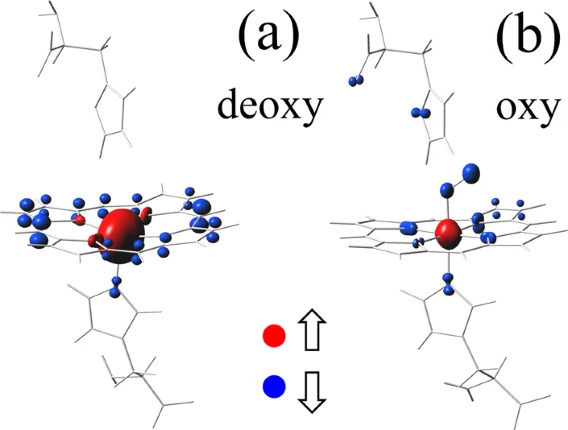
\includegraphics[width = 0.4\textwidth, height = 4.5cm]{assets/images/DeoxyHb_magnetic.jpg}
   \caption[Oxy- and Deoxy-hemoglobin Magnetic Moment Density]{Illustation of magnetic-moment density \textbf{M(r)} for the \textbf{(a)} \gls{HbR} and \textbf{(b)} \gls{HbO} heme clusters at \textit{T = 150K}. The magnitude of \textbf{M(r)} at an atomic site is proportional to the volume of the bubble at that site. Adapted from Fig. 2 p.2 \paper{Mayda}{Mayda2020}.}
   \label{fig:HbMagnetic}
\end{wrapfigure}

The combination of the aforementioned with the biophysical phenomenon, that when a brain area is activated, the blood flow increases-via a process called the hemodynamic response-to a greater degree than the oxygen metabolic rate, produces a useful basis for an experimental signal acquisition technique. The second phenomenon leads to a reduction in the \gls{OEF}, a seemingly paradoxical scenario in which the venous blood is more oxygenated, despite the increase in oxygen metabolic rate, because the blood flow has increased to a greater extent. Taken together, these two phenomena produce the \gls{BOLD} effect, a local increase in the \gls{MR} signal due to a reduction in the \gls{OEF} during increased neural activity. \cite{Buxton2013}

% Misconception tackled.
A prevailing misconception is that \gls{BOLD} provides a direct measurement of neuronal oxygen consumption. However, this is generally not the case; classic positive \gls{BOLD} signals, seen in response to functional stimuli, represent a decrease in \gls{HbR} and thus an overoxygenation of the responding region \cite{Attwell2002}. These positive \gls{BOLD} responses correspond to a local, actively actuated, increase in blood flow and volume, which brings blood in sufficient excess to increase local oxygenation levels \cite{Raichle1998}. This response typically begins within about 500ms and peaks 3 to 5 seconds after stimulus onset \autoref{fig:BOLD}, even for short stimuli lasting less than 1 second, with more complex dynamics for prolonged stimuli.

\begin{figure}[htbp]
    \centering
    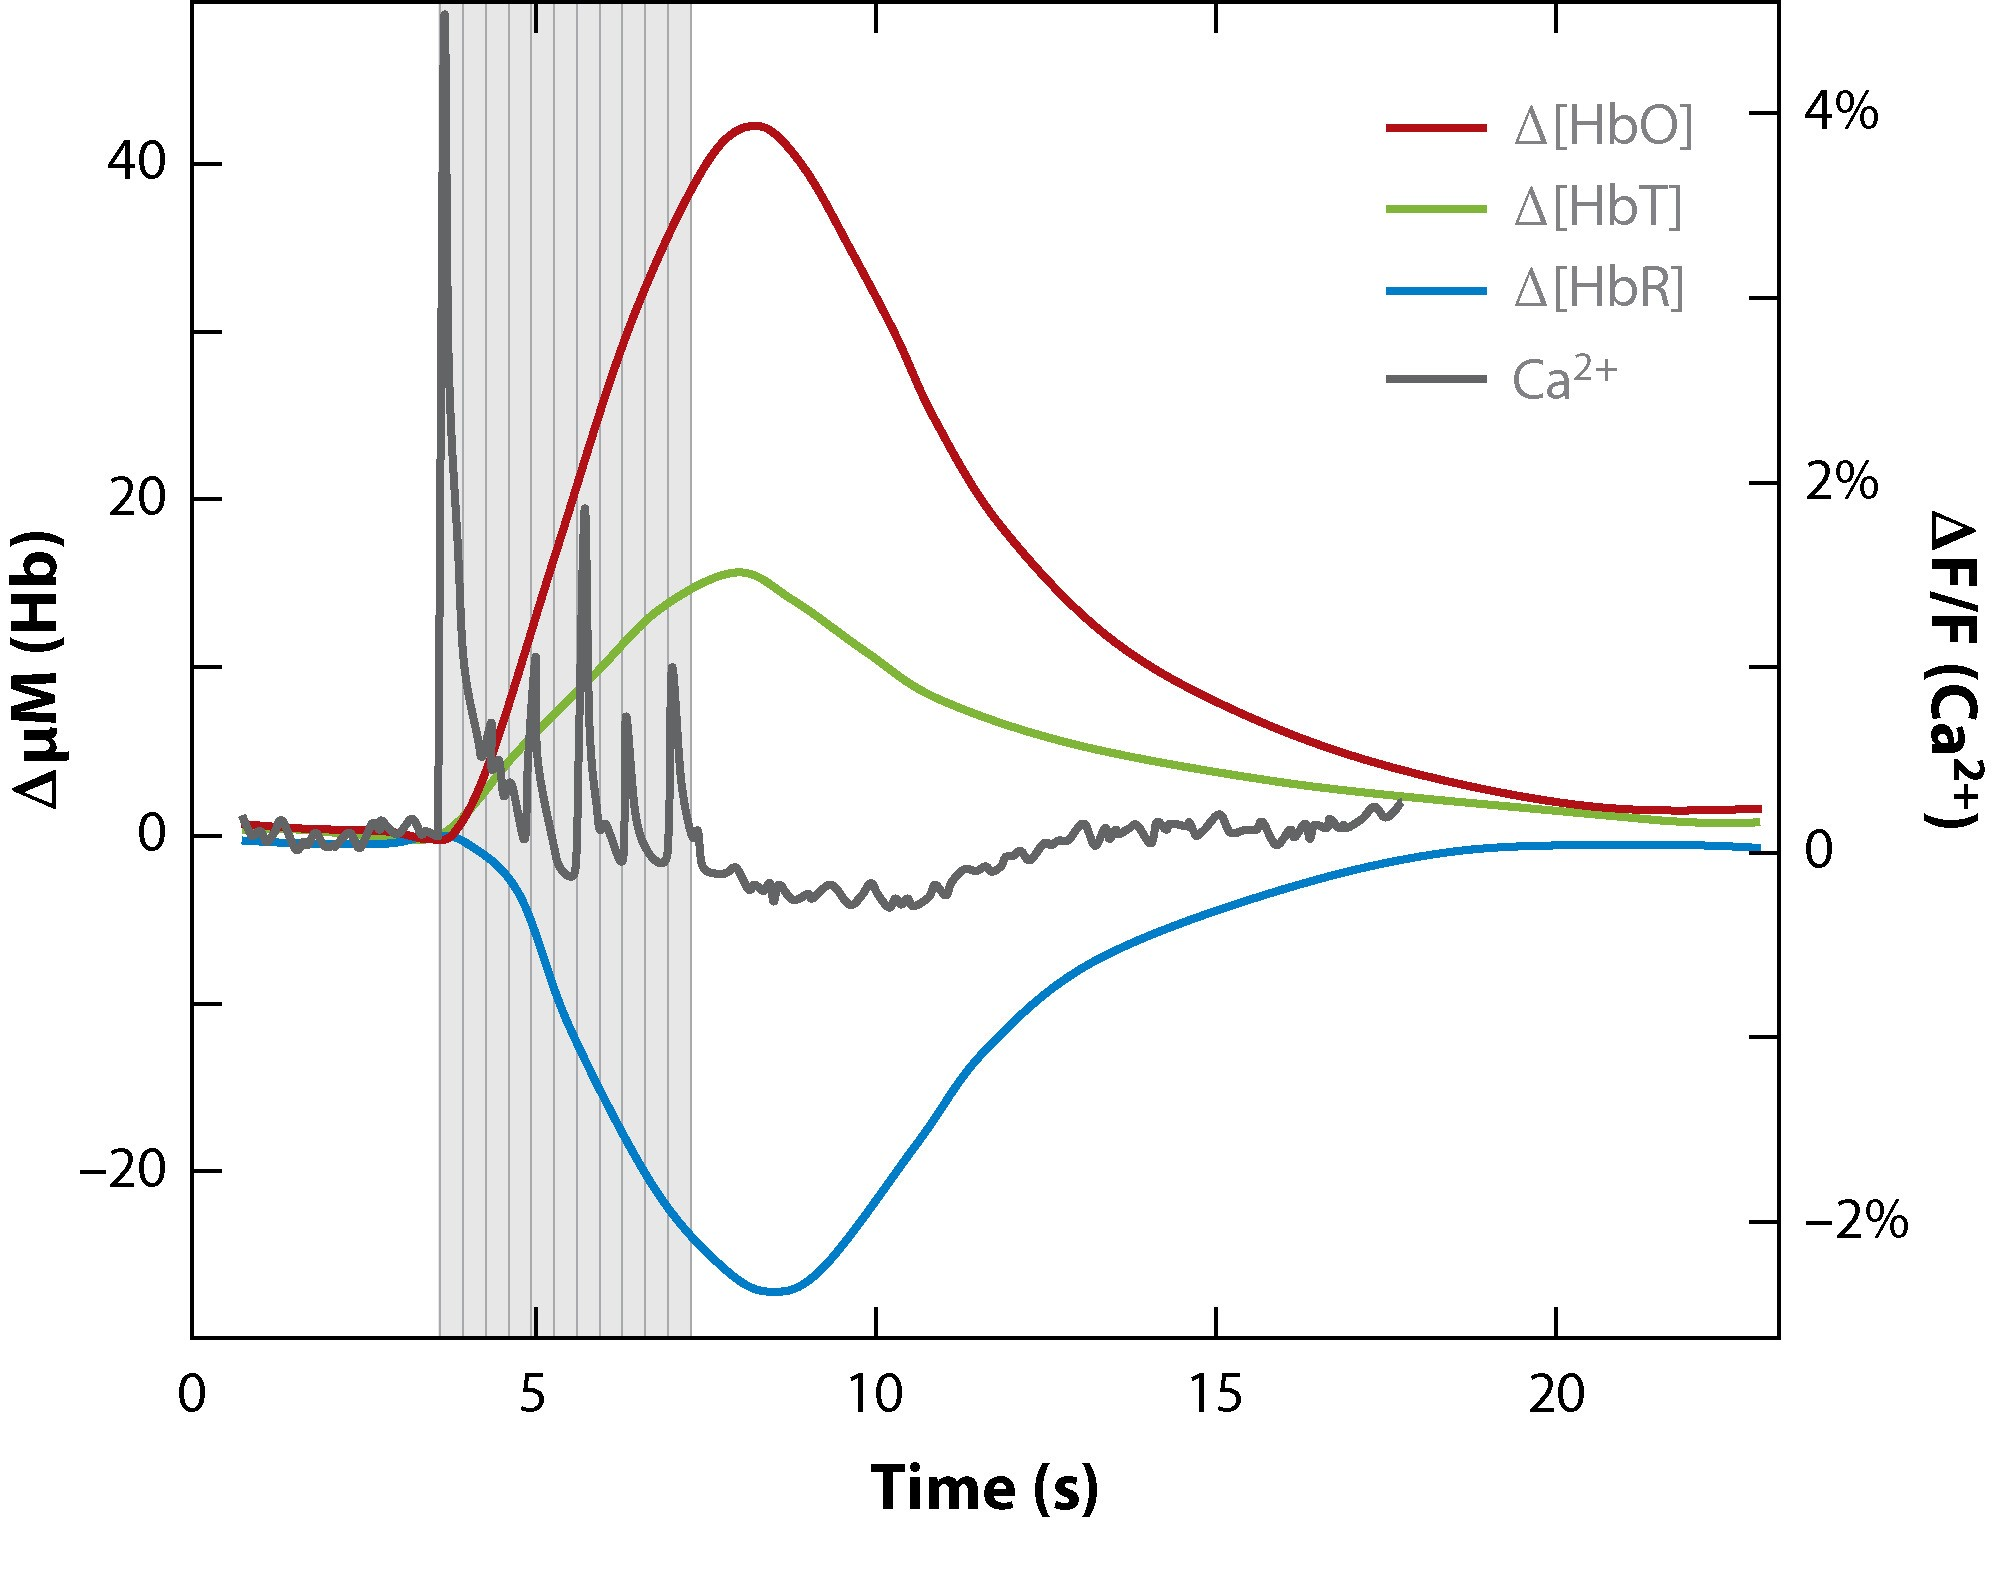
\includegraphics[width = 0.75\textwidth, height = 7cm]{assets/images/Hb_flactuations_BOLD.jpg}
    \caption[Stimulus-evoked Response in Somatosensory Cortex of Rats]{Stimulus-evoked response in somatosensory cortex of rats. Noteably, there is a distinct increase in \gls{HbT} corresponding to vessel dilation and an increase in the number of red blood cells per unit volume of cortex, consistent with an increase in blood flow. \gls{HbO} increases while \gls{HbR} decreases, indicating a net overoxygenation of the region. The \gls{fMRI} \gls{BOLD} is sensitive to changes in \gls{HbR}, where stimulus-evoked "positive \gls{BOLD}" corresponds to the decrease in \gls{HbR} shown here. Adapted from Fig. 2 p.4 \paper{Hillman}{Hillman2007}.}
    \label{fig:BOLD}
\end{figure}

% Broad finishing statements.
A range of cellular mechanisms, including astrocytes, pericytes, and interneurons, have been proposed to play a role in neurovascular coupling.\cite{Hillman2014}. For classical interpretation of \gls{BOLD} signals, it is assumed that neurovascular coupling is so robust that any increase in neuronal activity generates a proportional increase in local blood flow, irrespective of brain region, brain development, and pathological state \cite{Logothetis2010}.
\section{Data Acquisition and Manipulation}


\subsection{The Human Connectome Project (\textit{HCP})}

\begin{frame}
\frametitle{The Human Connectome Project (\textit{HCP})}
	\begin{itemize}
		\uncover<1->{\item Five-year effort to characterize brain connectivity, function\\and their variability in healthy adults}
		\uncover<2->{\item Multiple imaging modalities: dMRI, r-fMRI,\\t-fMRI, T1w and T2w MRI, MEG, and EEG}
		\uncover<3->{\item 1200 subjects, 300 sibships mostly including\\a mono- or di-zygotic twin pair}
	\end{itemize}
\end{frame}

%\begin{frame}
%\frametitle{HCP Image Acquisition Schematic Summary}
	%\begin{figure}
	%	\centering
	%	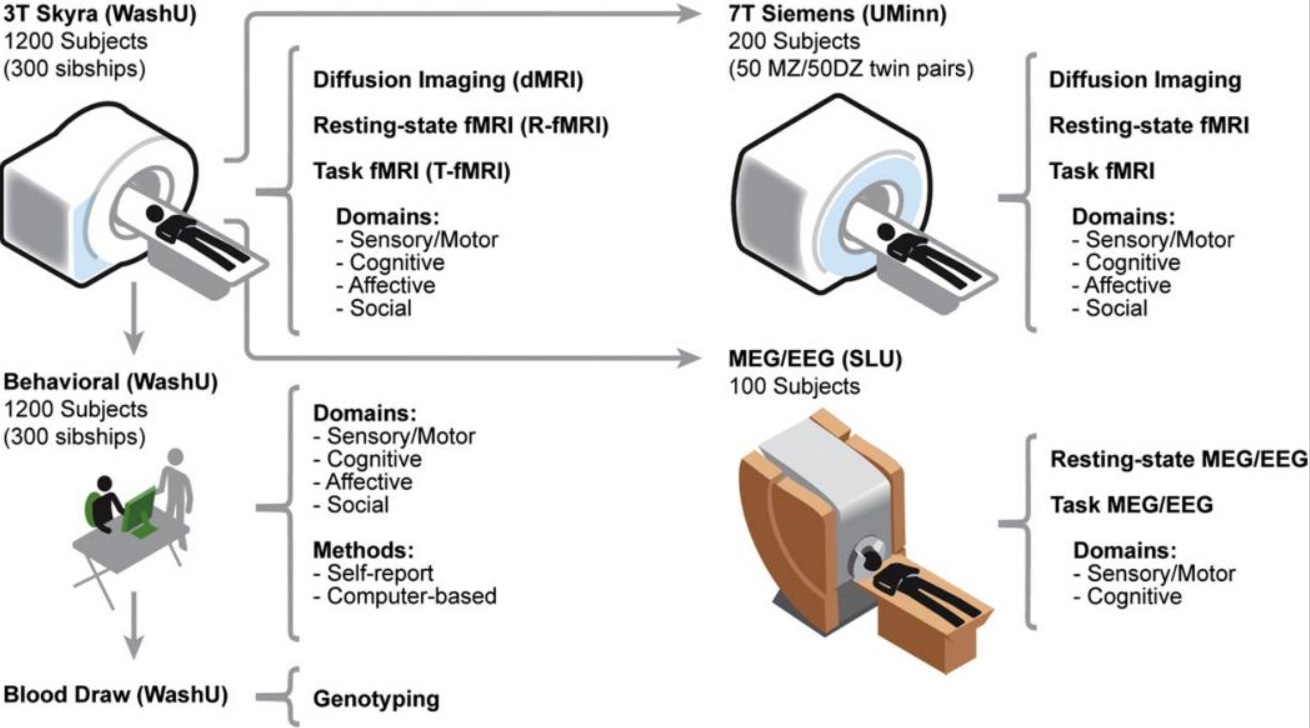
\includegraphics[width=0.98\textwidth]{assets/HCP_plan.png}
	%	\caption*{HCP Image Acquisition Schematic Summary}
	%\end{figure}
%\end{frame}


\subsection{Task-fMRI Battery of the HCP}

\begin{frame}
\frametitle{Task-fMRI Battery of the HCP}
	\text{Neural systems targeted by the tests:}
	\vspace{0.8cm}
	\begin{itemize}
		\item Visual and Somatosensory-Motor Systems
		\item \textbf{Category-Specific Representation}
		\item Language Function (semantic and phonological processing)
		\item Attention Systems
		\item \textbf{Working Memory/Cognitive Control System}
		\item Emotion Processing
		\item Decision-Making/Reward Processing
		\item Episodic Memory Systems
	\end{itemize}
\end{frame}

\begin{frame}
\frametitle{Working Memory Task}
	\begin{columns}
		\begin{column}{0.5\textwidth}
			\begin{itemize}
				\uncover<1->{\item Subjects presented with blocks of trials that consisted of pictures of places, tools, faces, and body parts}
				\uncover<2->{\item N-Back paradigm was utilized}
				\uncover<3->{\item Every 2 blocks separated\\by a fixation period}
				\uncover<4->{\item 8 blocks per run,\\2 runs per subject}
			\end{itemize}
		\end{column}

		\begin{column}{0.49\textwidth}
				\begin{figure}
					\centering
					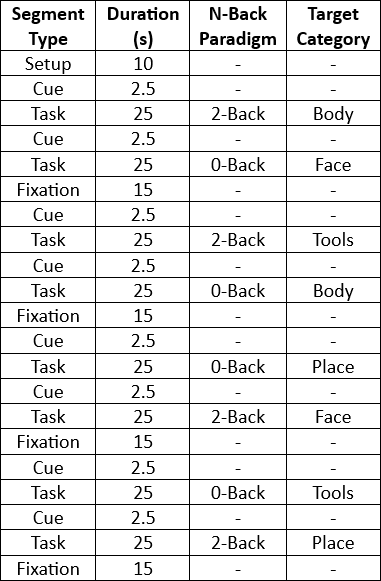
\includegraphics[width=\textwidth, height=6cm]{assets/WM_mat.png}
					\caption*{Sequence of WM Events}
				\end{figure}
		\end{column}
	\end{columns}	
\end{frame}


\subsection{Analysis of fMRI Signal}


\begin{frame}
\frametitle{The Hemodynamic Response Function}
	\begin{columns}
		\begin{column}{0.5\textwidth}
			\begin{itemize}
				\uncover<1->{\item Impulse stimulus produces\\acute hemodynamic response function (\textit{HRF})}
				\uncover<2->{\item Lasting stimulus produces boxcar HRF}
				\uncover<3->{\item HRF shape can be modelled with a Gamma Distribution}
			\end{itemize}
		\end{column}

		\begin{column}{0.49\textwidth}
			\only<1>{	
				\begin{figure}
					\centering
					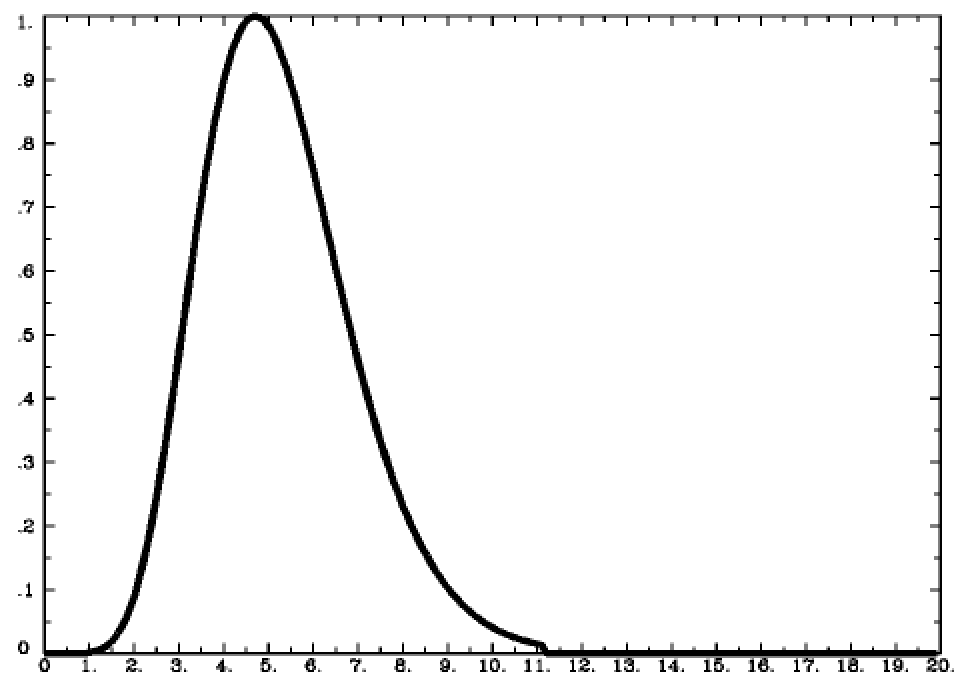
\includegraphics[width=\textwidth, height=6cm]{assets/single_HRF.jpg}
					\caption*{Illustration of Acute HRF.}
				\end{figure}
				}
			\only<2>{	
				\begin{figure}
					\centering
					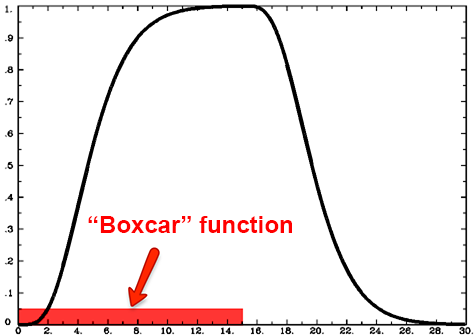
\includegraphics[width=\textwidth, height=6cm]{assets/box_HRF.jpg}
					\caption*{Illustration of Boxcar HRF.}
				\end{figure}
				}
			\only<3>{	
				\begin{figure}
					\centering
					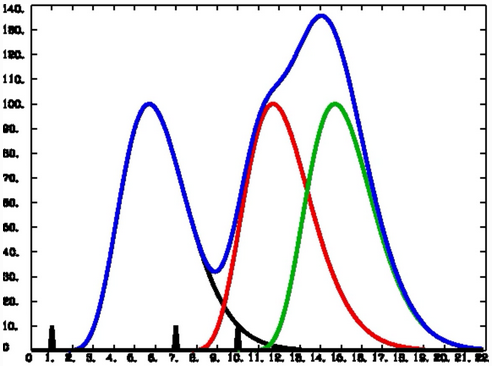
\includegraphics[width=\textwidth, height=6cm]{assets/overlap_HRF.png}
					\caption*{HRF Overlap and Fitting.}
				\end{figure}
				}
		\end{column}
	\end{columns}	
\end{frame}

% potential gif of hrf scaling

\begin{frame}
\frametitle{Analysis Process Overview}
	\begin{itemize}
		\uncover<1->{\item General Linear Model fitting to the BOLD signal time-series}
		\uncover<2->{\item Original explanatory variables (\textit{EV}) defined by the experiment}
		\uncover<3->{\item Beta-weights corresponding to each EV}
		\uncover<4->{\item Contrast of parameter estimates (\textit{COPE}) selected by researcher}
	\end{itemize}
	\begin{figure}
		\centering
		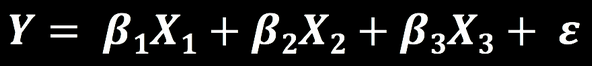
\includegraphics[width=\textwidth]{assets/glm.png}
	\end{figure}
\end{frame}

\begin{frame}
\frametitle{Unprocessed BOLD Time-Series.}
	\begin{itemize}
		\item Unprocessed BOLD Time-Series
	\end{itemize}
	\begin{figure}
		\centering
		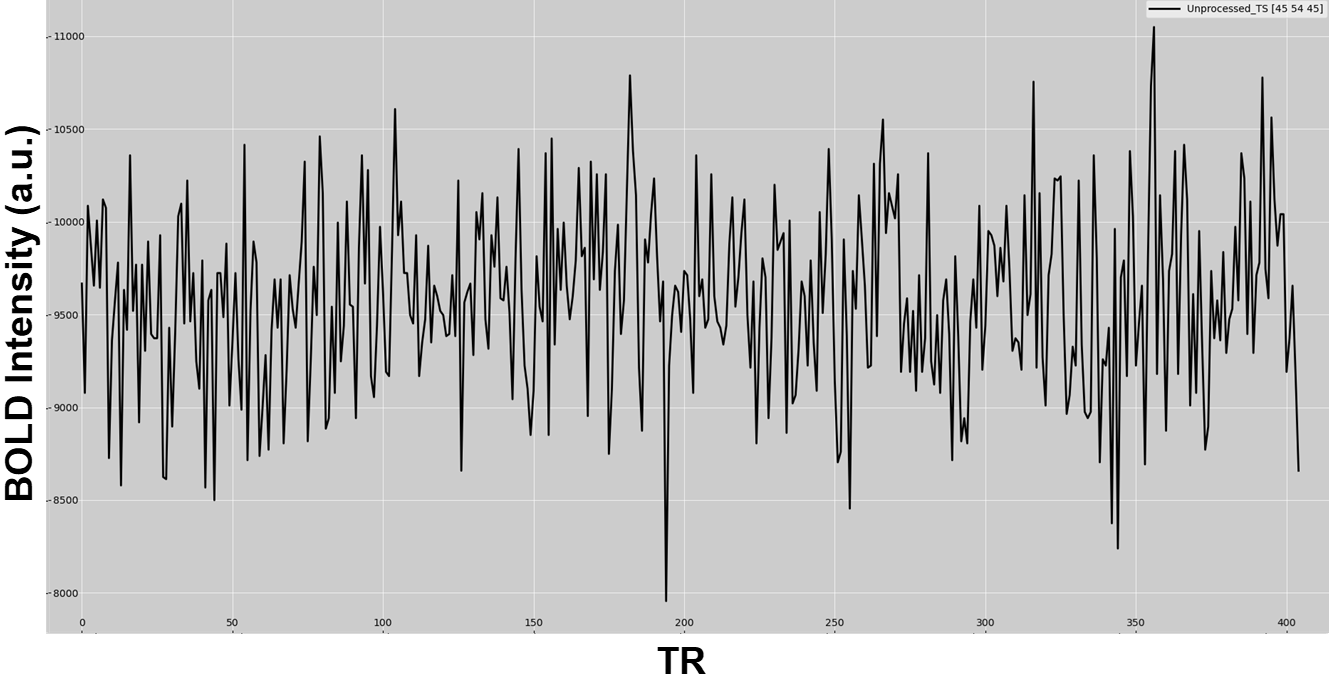
\includegraphics[width=\textwidth]{assets/unproc.png}
	\end{figure}
\end{frame}

\begin{frame}
\frametitle{Preprocessed BOLD Time-Series.}
	\begin{itemize}
		\item Unprocessed Versus Preprocessed BOLD Time-Series
	\end{itemize}
		\begin{figure}
			\centering
			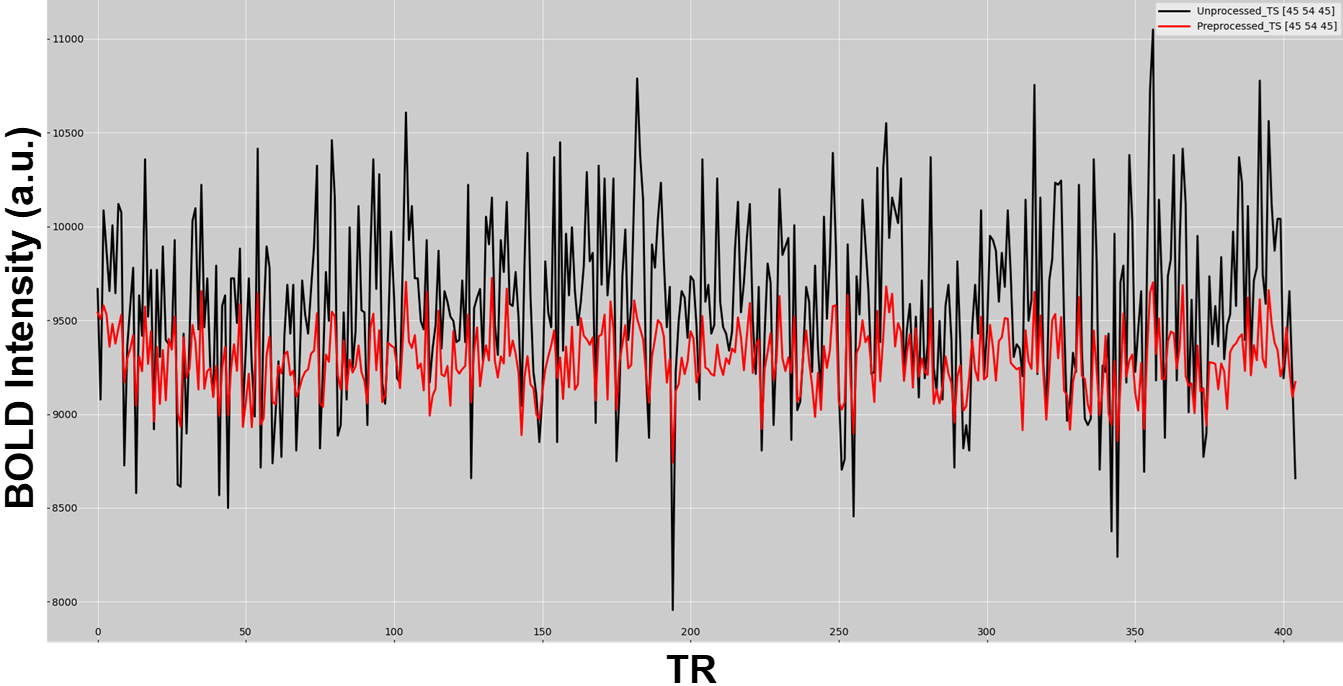
\includegraphics[width=\textwidth]{assets/preproc_and_unproc.png}
		\end{figure}
\end{frame}

\begin{frame}
\frametitle{Fitted BOLD Time-Series.}
	\begin{itemize}
		\item Preprocessed Versus Fitted BOLD Time-Series
	\end{itemize}
	\begin{figure}
		\centering
		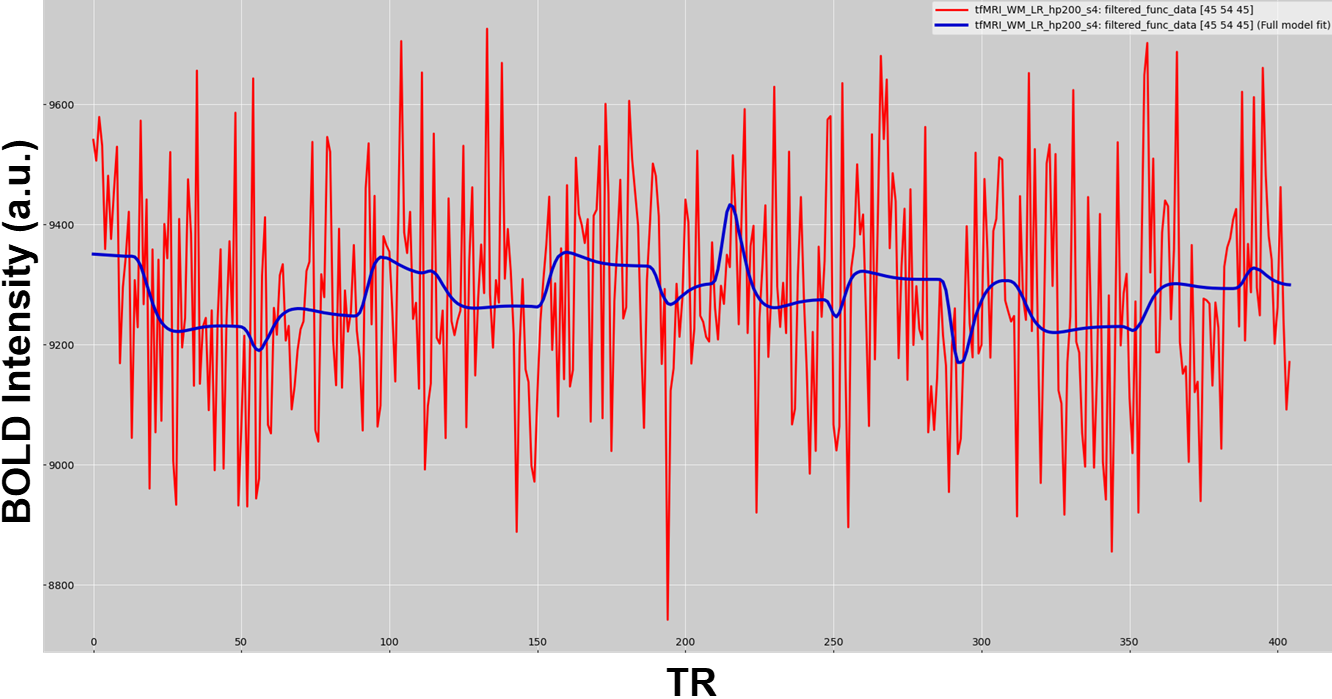
\includegraphics[width=\textwidth]{assets/fitted_and_preproc.png}
	\end{figure}
\end{frame}

%\begin{frame}
%\frametitle{Fitted BOLD Time-Series.}
%	\begin{itemize}
%		\item COPE configuration for estimating HRF beta weights for stimuli\\belonging to specific category and N-Back paradigm
%	\end{itemize}
%	\begin{figure}
%		\centering
%		\includegraphics[width=\textwidth]{assets/COPEs_4C.png}
%	\end{figure}
%\end{frame}
\pagebreak
\chapter{Methods}
\label{sec:methods}

\section{Pipeline Overview}

The procedure followed in the current work is displayed in figure \autoref{fig:pipeline}.

\begin{figure}[htbp]
    \centering
    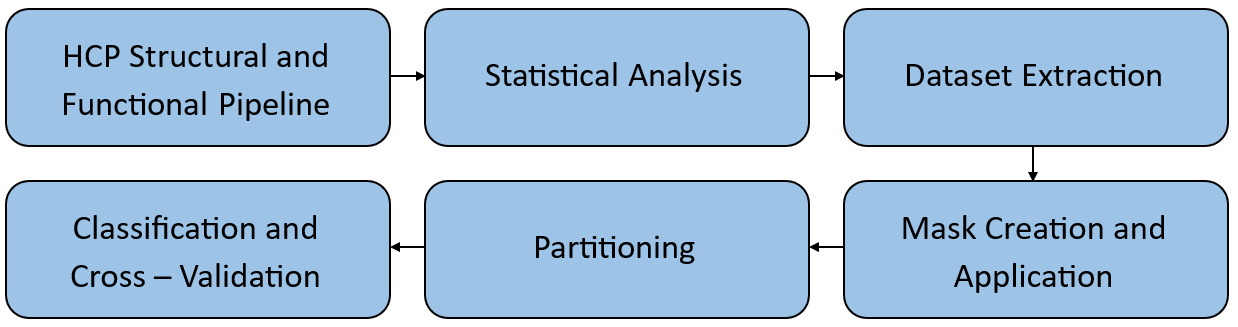
\includegraphics[width = 0.75\textwidth]{assets/images/pipeline.png}
    \caption[Pipeline Overview]{Pipeline Overview.}
    \label{fig:pipeline}
\end{figure}

\begin{wrapfigure}{r}{0.4\textwidth}
    \centering
    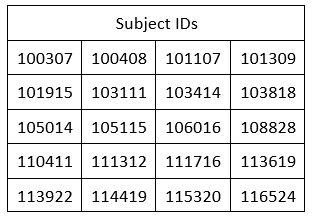
\includegraphics[width = 0.4\textwidth]{assets/images/IDs.png}
    \caption[]{List of IDs for subjects initially chosen for all analyses.}
    \label{fig:ids}
\end{wrapfigure}

% Manually add to the List of Tables and lower list of figures counter.
\addtocounter{table}{1}
\addcontentsline{lot}{table}{\protect\numberline{\thetable}Analysis Subject IDs}
\addtocounter{figure}{-1}

The starting point of the data was preprocessed \gls{WM} task \gls{fMRI} \gls{NIfTI} files, which had undergone initial pre-processing steps included in the structural and then functional \gls{HCP} pipelines \cite{Glasser2013} and were downloaded from the ConnectomeDB platform \cite{ConnectomeDB}. Twenty subjects, selected arbitrarily to balance a reasonable effect size with low computing power needs, were included as shown in figure \autoref{fig:ids}. For all analyses, \gls{NIfTI} files from both \gls{LR} and \gls{RL} scans were included for all subjects. This \gls{LR} and \gls{RL} distinction was made to facilitate geometric distortion correction while simultaneously providing additional data points.

\section{Pipeline Segments}

\subsection{Preprocessing}

All data processing was executed in FMRIB Software Library, abbreviated FSL (FSL v. 6.0.7.12, \cite{Jenkinson2012}). A single preprocessing setting was altered from those in the \gls{HCP} pipelines: the spatial smoothing parameter. The dimensions of the rectangular smoothed voxel neighborhoods were changed from \SI{5}{\milli\meter} to \SI{4}{\milli\meter}. This adjustment improves the singal-to-noise ratio and is a widely used standard for relatively small \gls{ROI}s, such as the \gls{FFA} and \gls{PPA}, which are examined in this study.

\subsection{Statistical Analysis}
\label{subs:stat}

Voxel-wise time-series were input into \gls{FEAT}. Based on the eight \gls{EV}s established by the \gls{HCP} pipeline (.fsf files) --- two \gls{EV}s for each stimulus category, one for 2-Back and one for 0-Back trials --- new \gls{COPE}s were designed. Two different analyses were conducted, both utilizing double-Gamma \gls{HRF} convolution fitting: 

\begin{figure}[htbp]
    \centering
    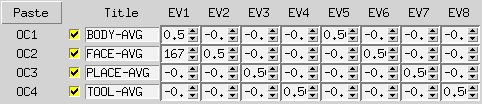
\includegraphics[width = 0.75\textwidth]{assets/images/COPEs_2C.png}
    \caption[]{List of \gls{COPE}s designed for all \gls{2C} analyses.}
    \label{fig:copes_2C}
\end{figure}

% Manually add to the List of Tables and lower list of figures counter.
\addtocounter{table}{1}
\addcontentsline{lot}{table}{\protect\numberline{\thetable}2C Analyses COPEs}
\addtocounter{figure}{-1}

\begin{enumerate}[label=\Roman*.]

\item In the first analysis, 4 \gls{COPE}s (see fig. \autoref{fig:copes_2C}) were parametrized to estimate the \gls{HRF} corresponding to the average \gls{BOLD} signal of each stimulus category, regardless of the N-Back paradigm used. The category-specific signal was averaged by including both 2-Back and 0-Back trials with equal weighting ($ 50 - 50 $), and the signal from all other trials was subtracted using a factor of $ -0.167$ $(1/6)$.

\item In the second case, the same approach was taken, but the signals from 2-Back and 0-Back trials for each stimulus category were considered independent, resulting in 8 \gls{COPE}s (see fig. \autoref{fig:copes_4C}). This decision was based on the fact that these blocks were always separated by tens of seconds. Thus, each \gls{EV}'s average signal was calculated while subtracting all other sources with a factor of $ -0.143$ $(1/7)$.

\end{enumerate}

\begin{figure}[htbp]
    \centering
    \includegraphics[width = 0.75\textwidth]{assets/images/COPEs_4C.png}
    \caption[]{List of \gls{COPE}s designed for all \gls{4C} analyses.}
    \label{fig:copes_4C}
\end{figure}

% Manually add to the List of Tables and lower list of figures counter.
\addtocounter{table}{1}
\addcontentsline{lot}{table}{\protect\numberline{\thetable}4C Analyses COPEs}
\addtocounter{figure}{-1}

A Unix shell script was created to automate \acrshort{FEAT} analyses across all runs of all available subjects. The script requires only the original .fsf file, which contains the analysis design, as input. In the first case, each analysis produced $4$ \gls{COPE}s, resulting in $4$ patterns per run (\gls{LR} and \gls{RL}) and $8$ patterns per subject, generating a total of $160$ patterns. In the second case, each analysis produced $8$ \gls{COPE}s, resulting in $8$ patterns per run (\gls{LR} and \gls{RL}) and $16$ patterns per subject, generating a total of $320$ patterns.

It is important to note that the \acrshort{FEAT} analysis is a single core process and the time required to complete is not bound on the number of \gls{COPE}s included, but rather on the complexity of the \gls{COPE} design and the quantity of voxels analysed. As a result, with the current hardware limitations and no parallel programming automation designed for this body of work, each analysis took an average of approximately 22 \si{\minute} in the first occasion and 16 \si{\minute} in the second, even though the number of \gls{COPE}s was doubled in the latter.

\subsection{Dataset Extraction - Construciton}

All subsequent data analysis was conducted using custom code written in MATLAB (R2023b). A script was developed to extract patterns from each run for each subject, scalable to accommodate any name and number of subjects. All patterns were conjoined into a single dataset, with sample attributes assigned to them, including target, target label and chunk. The target refers to the stimulus category, numbered as follows: 1 for Body, 2 for Face, 3 for Place, and 4 for Tool, with the labels being the human-readable target names. Chunks are distinguished by a unique number, denoting pattern independence. This independence is crucial because it allows the classifier to train and test on disjoint sets of chunks, thereby avoiding circular analysis (double-dipping).

The analysis that merges signal from 2-Back and 0-Back trials resulted in $2$ chunks per subject and shall be referred to as analysis \gls{2C}. The analysis that separates the signals from different N-Back paradigms produced $4$ chunks per subject and will therefore be called \gls{4C}.

\subsection{Mask Creation - Application}

Once the data was fully processed, two masks were created to distinguish data pertaining to the \gls{FFA} and the \gls{PPA}. These masks, which are logical matrices applied to the dataset to exclude any data outside the selected \gls{ROI}, were "circular", though pixelated, with a radius of $12$ voxels, containing a total of $1,416$ voxels. Mask centers were determined using Neurosynth's Locations Tool (see \cite{neurosynth}) and identified as [40, -52, -20] for the \gls{FFA} and [26, -33, -19] for the \gls{PPA}, in MNI152 coordinates. The radius was specifically chosen to maximize \gls{ROI} volume (ensuring the intended brain region is within the \gls{ROI} for all subjects) while preventing overlap between brain regions that process different category-specific information, as shown in figure (\autoref{fig:radius}).

\begin{figure}[htbp]
    \centering
    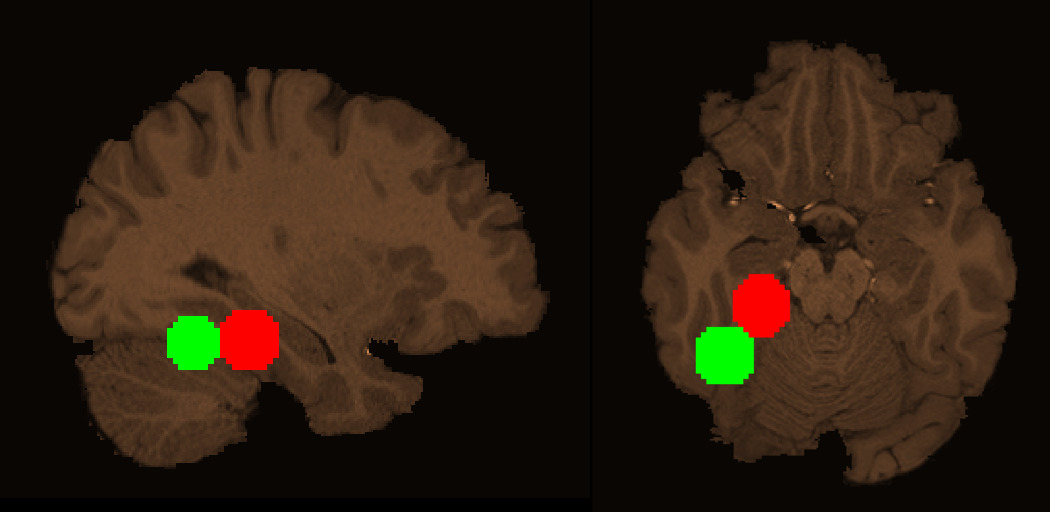
\includegraphics[width = 0.75\textwidth]{assets/images/masks_sag_trans.jpg}
    \caption[Illustration of FFA and PPA masks]{Illustration of \gls{FFA} and \gls{PPA} \gls{ROI}s after mask application, at the saggital and transverse planes. Notably, there is no overlap between the two areas, even when they are at their maximum extent.}
    \label{fig:radius}
\end{figure}

It should be noted that this is the first point at which the sheer volume of data can be reduced without loss of potentially crucial information. The initial dataset contained patterns for all $902.629$ voxels, depicting signal for the entire brain. After the \gls{FFA} and \gls{PPA} masks were applied, the non-zero signal voxels included in the masked datasets were $925$ and $888$ respectively, allowing for a much faster, more efficient and more intricate manipulation of the data.

\subsection{Partitioning of Masked Dataset}

For classification, the data must be split into independent training and test sets. A script was developed to partition the masked dataset with a variable train/test split ratio. To facilitate cross-validation, the script can produce a specified number of folds, each containing unique combinations of patterns within training and test datasets. The classifier can be run on any number of these partitions, resulting in a mean accuracy that reliably reflects the classifier's predictive ability, independent of any single partitioning scheme. Partitioning was conducted with the CoSMo \gls{MVPA} independent\_sample\_partitioner command \cite{cosmo1}, following the appropriate manipulation of the dataset.

\subsection{Classifier Training and Testing \textit{(MVPA)}}

Classification is a supervised machine learning method in which the model predicts the correct label for a given input based on an algorithm that recognizes patterns associated with each label. In this study, the classifier functions as an 'eager learner,' creating a model and making future predictions based on this model, rather than continuously comparing test data to training data. A descriptive illustration of the process can be seen in \autoref{fig:class}.

\begin{figure}[htbp]
    \centering
    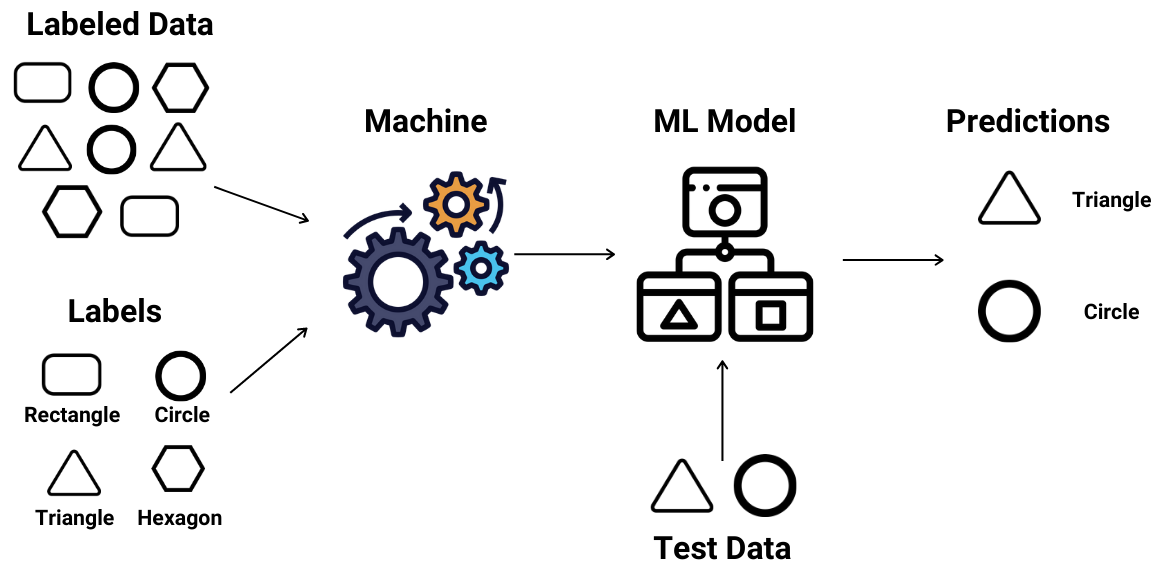
\includegraphics[width = 0.75\textwidth]{assets/images/class.png}
    \caption[Illustration of Supervised Learning Classification]{Supervised Learning Classificaiton Illustration. Adapted from \cite{ML}.}
    \label{fig:class}
\end{figure}

In this case, classification was conducted using the CoSMo \gls{MVPA} cosmo\_classify\_libsvm command \cite{cosmo2} which utilizes a \gls{SVM}  algorithm \cite{Cortes1995}.

\section{Data Analysis}

The classifier's accuracy was treated as a function of three variables, with all other parameters staying constant. The three variables were: 1) number of chunks of data per subject; 2) fold count; and 3) subject count.

\subsection{Category-Secific Baseline Brain Activation \textit{(UPA)}}

\glsreset{UPA}
The first step in facilitating further analysis is the \gls{UPA} of the baseline brain activation signal for each stimulus category in both regions. For each region, the statistical b-value assigned to each cope after the \acrshort{FEAT} analysis was used as an indicator of the baseline signal magnitude. The mean of the square of all values associated with each stimulus category was calculated to account for both positive and negative values. Consequently, the means for all \gls{2C} analyses were derived from 40 patterns, while for \gls{4C}, they were derived from 80 patterns, corresponding to the number of target-pattern pairs in each dataset. The results were presented in bar plots.

Additionally, an extra analysis was conducted for the \gls{FFA}, using cope values derived from a \acrshort{FEAT} analysis of a smaller, more central \gls{FFA} region with a radius of 6 voxels around the center, compared to the 12-voxel radius used previously. This approach aimed to clarify the relationships among the various signals, as they are expected to be more robust in this more focused area.

\subsection{Classifier Performance - Chunks per Subject}
\label{subs:ch_per_subj}

The \gls{WM} task paradigm used in the \gls{HCP} limits the maximum number of chunks per subject to 4, as trials within the same stimulation block (without intermittent fixation blocks) cannot be considered independent, and subjects participated in a total of 4 active trial blocks. However, the minimum number of chunks per subject can be as low as 1, effectively treating all trials as subject-dependent. The choice of chunk count depends on the researcher's approach and objectives.

\begin{enumerate}[label=\Roman*.]

\item In analysis \gls{4C} all blocks were considered independent as long as they involved a different N-Back paradigm and were separated by at least one fixation block. A total of 80 chunks were assigned to the 320 patterns, with each chunk containing 4 patterns, one for each target.

\item In analysis \gls{2C} the N-Back paradigm restriction was lifted. Signal from the same target's 2-Back and 0-Back blocks was placed in the same chunk, resulting in 40 chunks for all 320 patterns, with each chunk containing 8 patterns. Essentially, these chunks represent different runs, with two for each subject, totaling 40 chunks.

\end{enumerate}

\subsection{Detecting Outlier Subjects}
\label{subs:outliers}

The first step in data manipulation following \gls{FEAT} analyses was to identify any individual subjects whose data stood out as irregular. Considering our analysis focuses on the Fusiform Gyrus in the right hemisphere only, subjects who predominantly show activation in the left hemisphere could potentially dilute the classifier's data pool. The same issue can arise if a subject's data acquisition process contained artifacts. Determining outlier subjects is crucial before proceeding with further data analysis steps in order for the results to be reflective of the truth.

The 16 patterns corresponding to each subject in analysis \gls{4C} were individually run through the classifier, cross-validated with the maximum fold count of 4. In this process, 3 chunks (each containing 4 patterns) were used as training data, while the remaining chunk was utilized for testing. The mean accuracy of the classifier across all folds was calculated, and if it fell below 10\%, the subject was excluded from the remainder of the analysis, since such low accuracy is attributed to the nature of the data and not the classifier's properties. Consequently, two subjects were excluded from both the \gls{FFA} and the \gls{PPA} analyses, as further explained in \autoref{subs:res_outliers_ffa}.

These subject exclusions were applied to analysis \gls{2C} as well. Although the approach differs between N-Back trials for the same category-specific stimulus, the classifier's input remains fundamentally the same, so the characteristics that define a subject as an outlier are expected to remain consistent. Moreover, replicating the same analysis for \gls{2C} is impractical since each subject corresponds to only 8 patterns divided into 2 chunks. At best, this would allow for a 50/50 train/test split, where each dataset contains 4 patterns from different chunks. This split is far from ideal and does not accurately reflect the classifier's performance under the 80/20 ratio, which is utilized for all analyses to follow.

\subsection{Classifier Performance - Fold Count}

Cross-validation is essential for verifying the classifier's results, but it can also lengthen and complicate the process by introducing another variable: fold count. It's crucial to investigate this variable to determine the optimal number of folds for practical, repetitive analyses, as well as to identify the smallest number of folds at which the classifier's performance stabilizes. This allows us to estimate the maximum time required, even for high-precision analyses, ensuring efficiency without compromising accuracy.

Initially, \gls{4C} data was run through the classifier for all 18 subjects at high fold counts, starting at 250 and increasing up to 3000 in steps of 250 folds. The objective was to identify the cutoff point where performance stabilizes and further increasing the fold count no longer yields benefits. The accuracy metric at this stabilization point will be considered the objective accuracy of the classifier, serving as the benchmark to aim for at lower fold counts as well. Once the benchmark was established, the data was rerun through the classifier at fold counts ranging from 10 to 100. This approach not only highlights the classifier's performance at low, and therefore practical, fold counts but also helps identify the fold count at which the distribution of partitioning schemes closely resembles the one that produces the benchmark accuracy value. This allows for a more efficient yet accurate analysis by balancing practicality with precision. The same process was then repeated for \gls{2C} data. The optimal fold count was determined to be 68 folds for analysis \gls{4C} and 69 folds for analysis \gls{2C}. 

\subsection{Classifier Performance - Subject Count}

Another crucial variable to consider is the subject count. While accuracy is generally expected to improve as the number of subjects increases, provided they have been screened for outliers as shown in \autoref{subs:outliers}, it's important to determine the exact relationship between accuracy and subject count --- whether it is linear or more complex. Additionally, identifying if and when performance reaches an asymptote, and at what subject count or chunk count this practically occurs, is essential for optimizing the analysis without unnecessarily increasing the sample size.

A script was developed to automate the classification process for both \gls{4C} and \gls{2C} analyses across varying subject counts. For \gls{4C}, data from 1 to 18 subjects were sequentially fed into the classifier. When more than 2 subjects were involved, the optimal fold count of 68 was maintained. For 1 and 2 subjects, the fold count was set to the maximum possible, which was 4 and 28, respectively.

For \gls{2C}, the analysis for a single subject was skipped due to the limitations imposed by having only 2 chunks. The fold count was then set to 4, 15, 28, 45, and 66 for 2, 3, 4, 5, and 6 subjects, respectively, reflecting the maximum feasible number of folds for those subject counts. For all other subject counts, the fold count was standardized at 69.
\pagebreak
\chapter{Classification Results \& Discussion}
\label{sec:results}

%\section{Data Analysis - Results}

\section{Category-Secific Baseline Brain Activation \textit{(UPA)} - Results}

The average signal for faces in the \gls{FFA} is unexpectedly low (see \autoref{fig:upa_ffa}). However, this does not compromise the efficacy of \gls{MVPA}, as successful classification of category-specific signals relies on their patterns' distinctiveness from other signals, regardless of whether this distinction is due to signal strength or relative weakness. Nevertheless, this finding warrants further investigation.

\vspace{2pt}

\begin{figure}[htbp]
 	\centering
	\begin{subfigure}{0.49\textwidth}
		\centering
		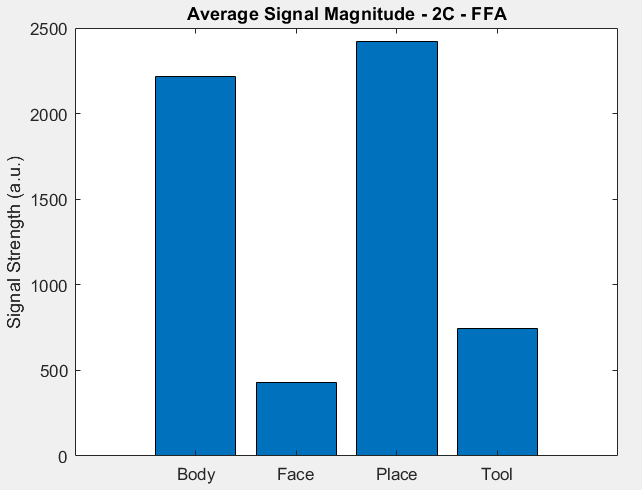
\includegraphics[width = 0.8\textwidth, height = 5cm]{assets/images/upa_2C_ffa.png}
		\caption{Average Magnitude of Brain Activation in the \gls{FFA} Across Different Stimulus Categories in the \gls{2C} Analysis.}
		\label{fig:upa_ffa_2C}
	\end{subfigure}
	\hfill
	\begin{subfigure}{0.49\textwidth}
		\centering
	 	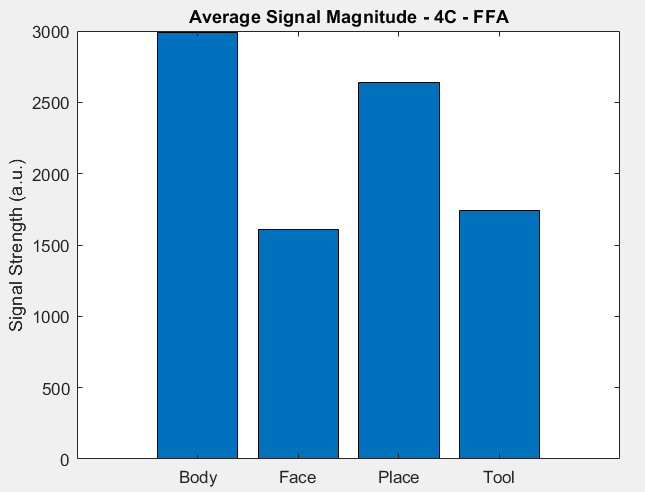
\includegraphics[width = 0.8\textwidth, height = 5cm]{assets/images/upa_4C_ffa.png}
		\caption{Average Magnitude of Brain Activation in the \gls{FFA} Across Different Stimulus Categories in the \gls{4C} Analysis.}
		\label{fig:upa_ffa_4C}
	\end{subfigure}
	\caption[Activation Magnitude Per Stimulus Category \textit{(UPA)} Bar Plots for the FFA]{Bar Plots Showing the Mean Activation for Each Stimulus Category Across the \gls{FFA}.}
 	\label{fig:upa_ffa}
\end{figure}

\vspace{2pt}

\begin{wrapfigure}{r}{0.4\textwidth}
    \centering
    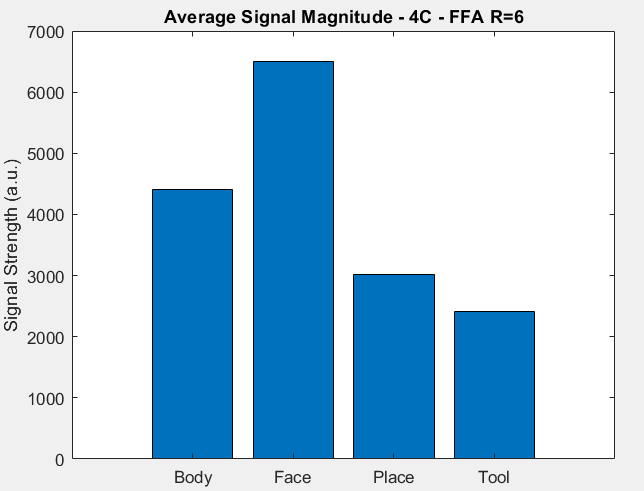
\includegraphics[width = 0.4\textwidth, height = 4.7cm]{assets/images/upa_4C_ffa_6.png}
    \caption[Activation Magnitude Per Stimulus Category \textit{(UPA)} Bar Plots for the FFA Centrally]{Bar Plots Showing the Mean Activation for Each Stimulus Category Across the \gls{FFA} When Mask Radius is 6.}
    \label{fig:upa_ffa_6}
\end{wrapfigure}

Examining the \gls{WM} task battery from which the data was derived, we observe that Faces were presented immediately after Bodies in the first instance and after Places in the second, never directly following a fixation phase. This sequence likely resulted in residual signals from the preceding stimulus categories, which could explain the magnitude observed for Bodies and Places. However, this does not account for the higher magnitude of Tools, which, theoretically, should not surpass that of Faces. A closer examination of the more central portion of the \gls{FFA} (see \autoref{fig:upa_ffa_6}), where residual overlap from other sources is minimized, reveals the expected signal profile: Faces show the highest activation magnitude, with Tools displaying roughly the same relative amplitude. This observation supports the earlier hypothesis and confirms that \gls{MVPA} can proceed using the initial, full \gls{FFA} mask.

In contrast, the signal in the \gls{PPA} is substantially higher for places than other stimuli (see \autoref{fig:upa_ppa}) throughout the whole region. The category-specific signals also tend to be ranked according to the proximity of their corresponding areas to the \gls{PPA}, suggesting that the differences in baseline signal may be due to overlap from place stimuli.

\begin{figure}[htbp]
 	\centering
	\begin{subfigure}{0.49\textwidth}
		\centering
		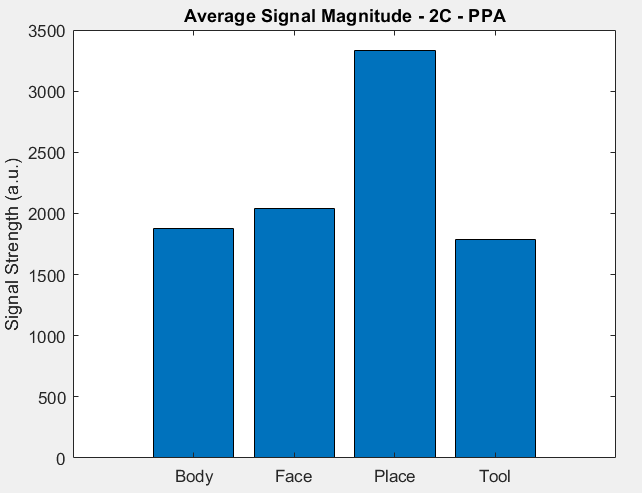
\includegraphics[width = 0.8\textwidth, height = 5cm]{assets/images/upa_2C_ppa.png}
		\caption{Average Magnitude of Brain Activation in the \gls{PPA} Across Different Stimulus Categories in the \gls{2C} Analysis..}
		\label{fig:upa_ppa_2C}
	\end{subfigure}
	\hfill
	\begin{subfigure}{0.49\textwidth}
		\centering
	 	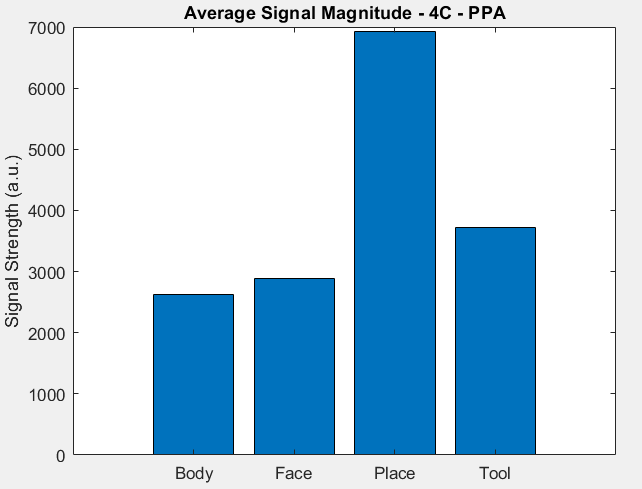
\includegraphics[width = 0.8\textwidth, height = 5cm]{assets/images/upa_4C_ppa.png}
		\caption{Average Magnitude of Brain Activation in the \gls{PPA} Across Different Stimulus Categories in the \gls{4C} Analysis..}
		\label{fig:upa_ppa_4C}
	\end{subfigure}
	\caption[Activation Magnitude Per Stimulus Category \textit{(UPA)} Bar Plots for the PPA]{Bar Plots Showing the Mean Activation for Each Stimulus Category Across the \gls{PPA}.}
 	\label{fig:upa_ppa}
\end{figure}

Notably, Places were presented once after a fixation phase and once after Tools, ensuring that the resulting signal is more canonical. As a result, the classifier is likely to perform better for place stimuli, although this will ultimately be confirmed or disproven by \gls{MVPA}.




%%% Start of FFA %%%




\section{Fusiform Face Area MVPA - Results}

\glsreset{FFA}
These are the classifier's performance results for the \gls{FFA}, analyzed across different variables.

\subsection{Chunks Per Subject \textit{(FFA)} - Results}

Using \gls{2C} data, the classifier achieved an optimal mean accuracy of 70\% across 3000 folds in the \gls{FFA}, while performance with \gls{4C} data capped at 61.9\%. The distributions of accuracies across folds were tested for normality, and a Lilliefors test confirmed that the data did not follow a normal distribution, with p-values of $1^{-3}$ for both datasets. Given that the two distributions also differed in variances, as shown by a two-sample F-test with a p-value of $<10^{-16}$, a Wilcoxon Rank-Sum test was conducted. The discrepancy between means was found to be statistically significant, with a p-value of $<10^{-16}$, undoubtedly confirming that the different approaches yielded distinct results and that the two analyses should be examined separately.

\subsection{Outlier Subjects \textit{(FFA)} - Results}
\label{subs:res_outliers_ffa}

After the classifier ran on each subject's data separately, using the maximum number of folds (4), the mean accuracies for each subject were calculated. As expected, these accuracies were generally lower than those obtained when the classifier was fed larger datasets. When all 20 subjects were included individually, the mean accuracy was 50\%, with a median value of 56.3\% (see \autoref{fig:per_subj_all_ffa}). However, two cases stood out immediately: Subject 100408 had a surprising accuracy of 0\%, and Subject 116524 showed an accuracy of 6.25\%. Given that the classifier completely failed to identify category-specific neural patterns in the first subject's data, it was assumed that the data was faulty for this analysis, and this subject was excluded from further steps. However, no robust reasoning was found to classify the second subject as an outlier, so they were included in the analysis.

\begin{figure}[htbp]
 	\centering
	\begin{subfigure}{0.49\textwidth}
		\centering
		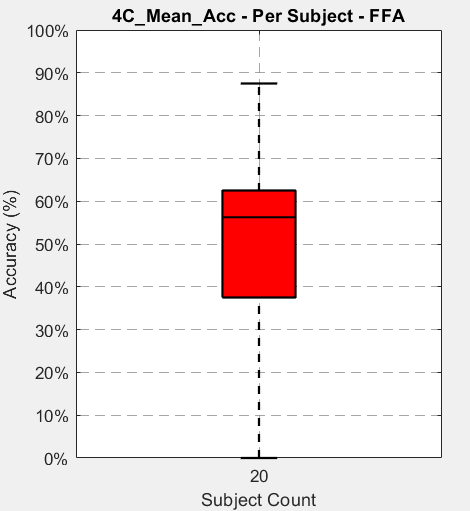
\includegraphics[width = 0.9\textwidth, height = 5cm]{assets/images/per_subj_4C_20_ffa.png}
		\caption{Boxplot Illustrating the Distribution of Initial Accuracy Across Individual Subjects.}
		\label{fig:per_subj_all_ffa}
	\end{subfigure}
	\hfill
	\begin{subfigure}{0.49\textwidth}
		\centering
	 	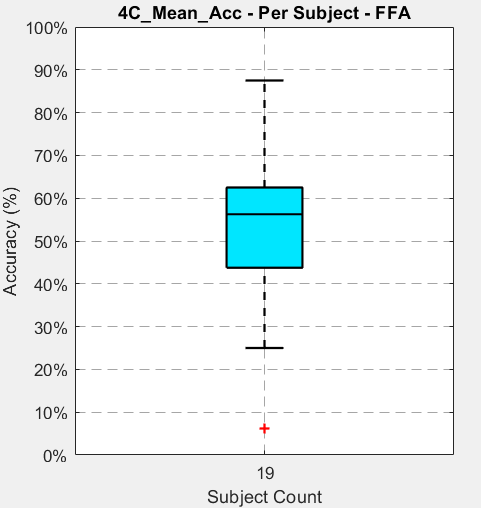
\includegraphics[width = 0.9\textwidth, height = 5cm]{assets/images/per_subj_4C_19_ffa.png}
		\caption{Boxplot Illustrating Accuracy Variance Across Individual Subjects After Excluding Outliers.}
		\label{fig:per_subj_19_ffa}
	\end{subfigure}
	\caption[Individual Subjects' Accuracies Boxplots for the FFA]{Boxplots Generated from the 'Per Subject' Analysis in the \gls{FFA}.}
 	\label{fig:per_subj_ffa}
\end{figure}

Once the outlier was removed, the mean accuracy for analyses involving one subject at a time increased to 52.6\%, with the median remaining constant (see \autoref{fig:per_subj_19_ffa}). Normally, this was still lower than the classifier's maximum potential accuracy of 61.9\%, which can be attributed to the low fold count used in these analyses. These results clearly indicate that screening for outlier subjects is crucial, as their inclusion can significantly impact the classifier's performance, particularly when working with smaller subject pools.

\subsection{Fold Count \textit{(FFA)} - Results}

The initial analysis, which focused on high fold counts, showed that accuracy stabilized to the second decimal point by 250 folds for both \gls{4C} and \gls{2C} analyses. This stability was reflected in the standard deviations of the distributions, which were 0.15\% for \gls{4C} and 0.17\% for \gls{2C}. In both cases, accuracy was slightly overestimated in the lower fold range of 250–1000, but eventually plateaued over 2500 folds, reaching 61.9\% for \gls{4C} and 70\% for \gls{2C}. These values represent the classifier's true accuracy and serve as the benchmarks to aim for in more practical, lower fold count analyses.

\begin{figure}[htbp]
 	\centering
	\begin{subfigure}{0.49\textwidth}
		\centering
		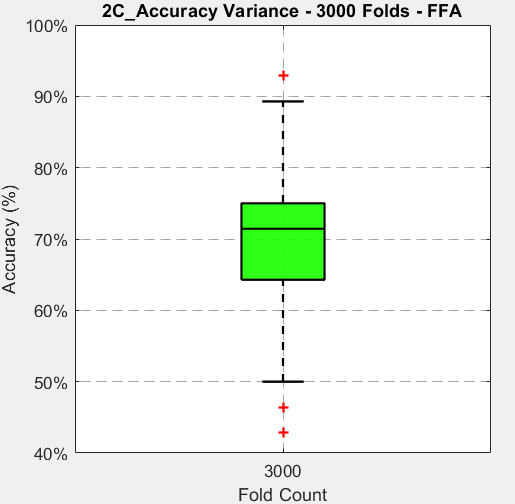
\includegraphics[width = 0.9\textwidth, height = 5cm]{assets/images/box_2C_3000_ffa.png}
		\caption{Accuracy Variance Across 3000 Folds for \gls{2C} Data.}
		\label{fig:2C_3000_ffa}
	\end{subfigure}
	\hfill
	\begin{subfigure}{0.49\textwidth}
		\centering
	 	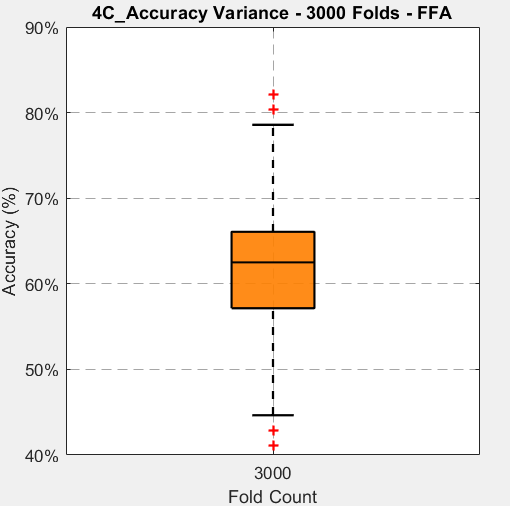
\includegraphics[width = 0.9\textwidth, height = 5cm]{assets/images/box_4C_3000_ffa.png}
		\caption{Accuracy Variance Across 3000 Folds for \gls{4C} Data.}
		\label{fig:4C_3000_ffa}
	\end{subfigure}
	\caption[Accuracies Across 3000 Folds Boxplots For The FFA]{Boxplots Produced During the 'High Number of Folds' Analysis in the \gls{FFA}.}
 	\label{fig:fold_HN_ffa}
\end{figure}

Furthermore, \autoref{fig:fold_HN_ffa} presents a boxplot for both analyses, illustrating the spread of accuracies across all 3000 folds. This distribution of partitions drives the classifier to its benchmark performance. To establish a practical fold count, the partitioning scheme distribution should mimic the one shown in the boxplot. This rationale led to the optimal practical fold count values being set at 69 for \gls{2C} and 68 for \gls{4C}.

\begin{figure}[htbp]
 	\centering
	\begin{subfigure}{0.49\textwidth}
		\centering
		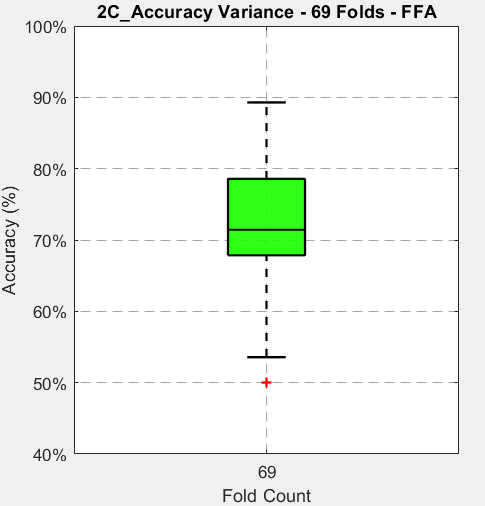
\includegraphics[width = 0.9\textwidth, height = 5cm]{assets/images/box_2C_69_ffa.png}
		\caption{Accuracy Variance Across the Optimal 69 Folds for \gls{2C} Data.}
		\label{fig:2C_69_ffa}
	\end{subfigure}
	\hfill
	\begin{subfigure}{0.49\textwidth}
		\centering
	 	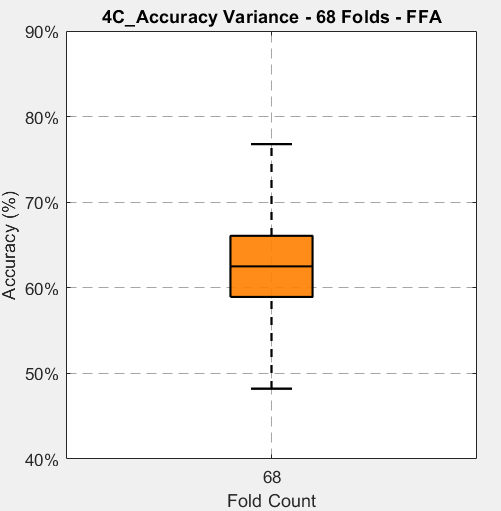
\includegraphics[width = 0.9\textwidth, height = 5cm]{assets/images/box_4C_68_ffa.png}
		\caption{Accuracy Variance Across the Optimal 68 Folds for \gls{4C} Data.}
		\label{fig:4C_68_ffa}
	\end{subfigure}
	\caption[Accuracies At Optimal Fold Count Boxplots For The FFA]{Boxplots Produced During the 'Practical Fold Count' Analysis in the \gls{FFA}.}
 	\label{fig:fold_ffa}
\end{figure}

The boxplots illustrated in \autoref{fig:fold_ffa} demonstrate distributions that closely resemble those obtained from the 3000-fold count analysis. These results indicate that the practical fold count approach provides both high accuracy and efficiency, making it a viable alternative for repeated analyses without compromising on the classifier's performance. The similarity in distributions confirms that reducing the number of folds to a more manageable level does not significantly affect the accuracy of the results.

\subsection{Subject Count \textit{(FFA)} - Results}

In the context of the \gls{2C} analysis, \autoref{fig:count_2C_ffa} shows that with just 2 subjects included, the classifier is already performing at a 50\% success rate. As more subjects are added, accuracy naturally increases, oscillating within the 65-70\% range, and eventually approaches the classifier's true potential accuracy of 70\% with 19 subjects included. The only truly irregular data point occurs at 4 subjects, where the classifier achieves a 78.1\% success rate. This anomaly can be attributed to the low number of data points in the analysis at this stage, combined with the necessarily low fold counts used in low subject counts analyses, and does not reflect a realistic performance for the classifier.

\begin{figure}[htbp]
 	\centering
	\begin{subfigure}{0.49\textwidth}
		\centering
		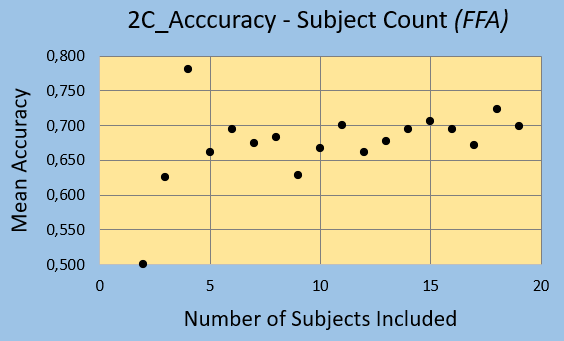
\includegraphics[width = 0.9\textwidth, height = 5cm]{assets/images/subj_count_2C_ffa.png}
		\caption{Accuracy Variance Across Different Subject Counts for \gls{2C} Data.}
		\label{fig:count_2C_ffa}
	\end{subfigure}
	\hfill
	\begin{subfigure}{0.49\textwidth}
		\centering
	 	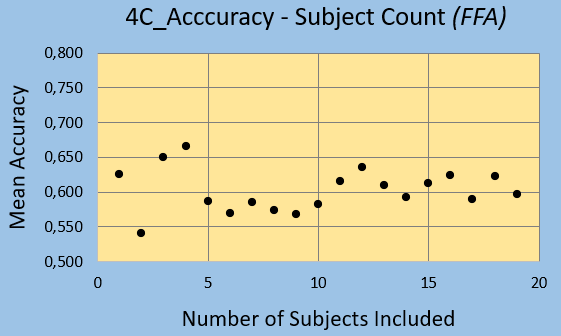
\includegraphics[width = 0.9\textwidth, height = 5cm]{assets/images/subj_count_4C_ffa.png}
		\caption{Accuracy Variance Across Different Subject Counts for \gls{4C} Data.}
		\label{fig:count_4C_ffa}
	\end{subfigure}
	\caption[Accuracies Across Subject Counts For The FFA]{Data Produced During the 'Subject Count' Analysis in the \gls{FFA}.}
 	\label{fig:count_ffa}
\end{figure} 

The same behavior is observed for the \gls{4C} analysis (see \autoref{fig:count_4C_ffa}). The overly high accuracy pattern at 3 and 4 subjects is repeated, further supporting the idea that brain activation patterns and partitioning schemes at this stage are overly favorable for the classifier. Additionally, another irregular point is observed at a subject count of 1, which was not feasible in the previous analysis. In this case, the fold count is only 4, and the potential performance outcomes are too limited to be truly representative. Therefore, interpreting the data at such low subject counts holds little value.

In both cases, accuracy appears to reach realistic values with at least 5 subjects, showing 66.1\% compared to the optimal 69.9\% for the \gls{2C} analysis and 58.7\% compared to the optimal 59.7\% for the \gls{4C} analysis.

The reasons behind this behavior of the classifier can only be speculated, as the baseline signal appears irregular (see \autoref{fig:upa_ffa}). A likely explanation is that the rapid stabilization of the classifier's accuracy is not so much a positive sign, as it indicates not that the classifier achieves high success rates at low subject counts but instead that it fails to increase success rate with additional data points. This could be due to the mixed nature of the baseline signal resulting in the disparity among stimuli categories being potentially, yet unpredictably, extenuated as more subjects are included in the analysis.





%%% Switch from FFA to PPA %%%





\section{Parahippocampal Place Area MVPA - Results}

\glsreset{PPA}
These are the classifier's performance results for the \gls{PPA}, analyzed across different variables.

\subsection{Chunks per Subject \textit{(PPA)} - Results}

In the analysis involving 3000 folds in the \gls{PPA}, the classifier achieved 66.4\% accuracy using \gls{2C} data and 50.6\% with \gls{4C} data, highlighting an even larger gap between the two approaches than in the \gls{FFA}. A Lilliefors test rejected the null hypothesis of normality for both datasets, with p-values of $1^{-3}$. The variance between the two datasets was also significantly different, as confirmed by a two-sample F-test with a p-value of $<10^{-16}$. Finally, the Wilcoxon Rank-Sum test returned a p-value of absolute zero, indicating that it was too low for MATLAB to compute a precise result. This confirms that the two distributions differ significantly and should be investigated separately.

\subsection{Outlier Subjects \textit{(PPA)} - Results}
\label{subs:res_outliers_ppa}

In this case individual accuracy scores were far lower than the classifier's optimal performance, with only three out of twenty cases surpassing it, as indicated by the overall mean accuracy of 32.5\% when all subjects were included with a median of 34.4\% (see \autoref{fig:per_subj_all_ppa}).

\begin{figure}[htbp]
 	\centering
	\begin{subfigure}{0.49\textwidth}
		\centering
		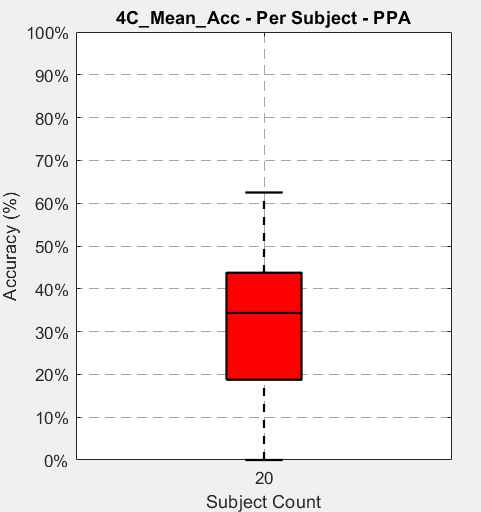
\includegraphics[width = 0.9\textwidth, height = 5cm]{assets/images/per_subj_4C_20_ppa.png}
		\caption{Boxplot Illustrating the Distribution of Initial Accuracy Across Individual Subjects.}
		\label{fig:per_subj_all_ppa}
	\end{subfigure}
	\hfill
	\begin{subfigure}{0.49\textwidth}
		\centering
	 	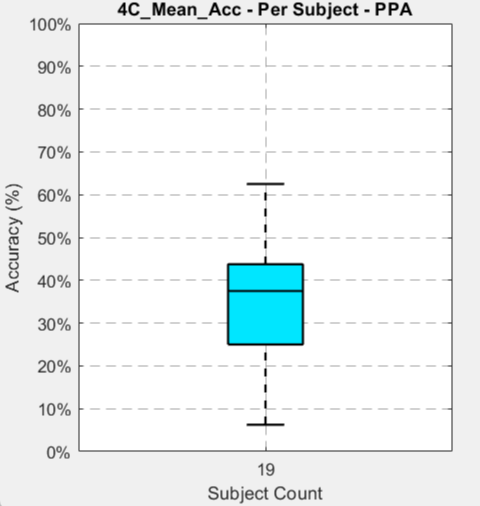
\includegraphics[width = 0.9\textwidth, height = 5cm]{assets/images/per_subj_4C_19_ppa.png}
		\caption{Boxplot Illustrating Accuracy Variance Across Individual Subjects After Excluding Outliers.}
		\label{fig:per_subj_19_ppa}
	\end{subfigure}
	\caption[Individual Subjects' Accuracies Boxplots for the PPA]{Boxplots Generated from the 'Per Subject' Analysis in the \gls{PPA}.}
 	\label{fig:per_subj_ppa}
\end{figure}

The same Subject 100408 produced an accuracy of 0\% again, further enhancing the notion that the specific subject's data potentially includes artifacts or irregularities. Once the outlier subject was excluded, mean accuracy rose to 34.2\% with a median of 37.5\% (see \autoref{fig:per_subj_19_ppa}).

\subsection{Fold Count \textit{(PPA)} - Results}

In both high fold count analyses, accuracy again stabilized to the second decimal point by 250 folds. In the \gls{4C} analysis, there was also stabilization to the third decimal point by 750 folds, with standard deviations of 0.12\% and 0.07\%, for \gls{2C} and \gls{4C} respectively. In the \gls{2C} case, accuracy at low fold counts was slightly lower than the final accuracy ultimately achieved by 2250 folds, which was 66.4\%, while with \gls{4C} data, accuracy remained practically stable throughout, at 50.6\%.

\begin{figure}[htbp]
 	\centering
	\begin{subfigure}{0.49\textwidth}
		\centering
		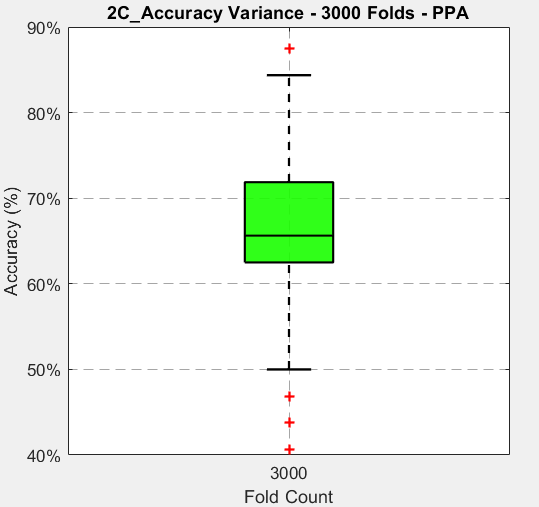
\includegraphics[width = 0.9\textwidth, height = 5cm]{assets/images/box_2C_3000_ppa.png}
		\caption{Accuracy Variance Across 3000 Folds for \gls{2C} Data.}
		\label{fig:2C_3000_ppa}
	\end{subfigure}
	\hfill
	\begin{subfigure}{0.49\textwidth}
		\centering
	 	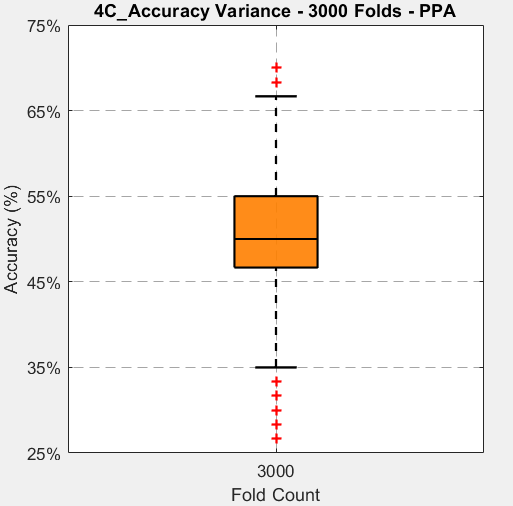
\includegraphics[width = 0.9\textwidth, height = 5cm]{assets/images/box_4C_3000_ppa.png}
		\caption{Accuracy Variance Across 3000 Folds for \gls{4C} Data.}
		\label{fig:4C_3000_ppa}
	\end{subfigure}
	\caption[Accuracies Across 3000 Folds Boxplots For The PPA]{Boxplots Produced During the 'High Number of Folds' Analysis in the \gls{PPA}.}
 	\label{fig:fold_HN_ppa}
\end{figure}

\autoref{fig:fold_HN_ppa} showcases the spread of accuracies across all 3000 folds for both analyses, indicating the distribution that should be sought after at low fold counts as well. With these in mind, the optimal practical fold count for \gls{2C} was set at 49 and for \gls{4C} at 62.

\begin{figure}[htbp]
 	\centering
	\begin{subfigure}{0.49\textwidth}
		\centering
		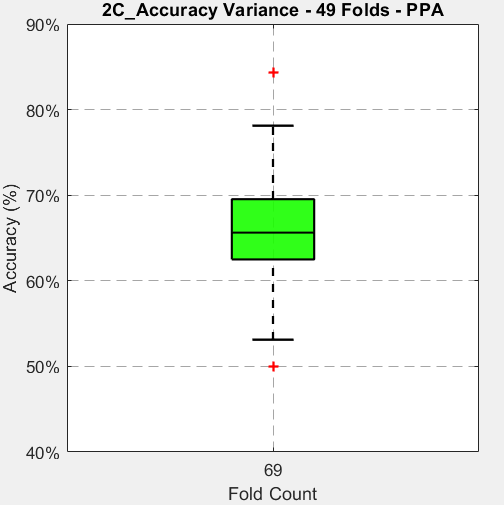
\includegraphics[width = 0.9\textwidth, height = 5cm]{assets/images/box_2C_49_ppa.png}
		\caption{Accuracy Variance Across the Optimal 49 Folds for \gls{2C} Data.}
		\label{fig:2C_49_ppa}
	\end{subfigure}
	\hfill
	\begin{subfigure}{0.49\textwidth}
		\centering
	 	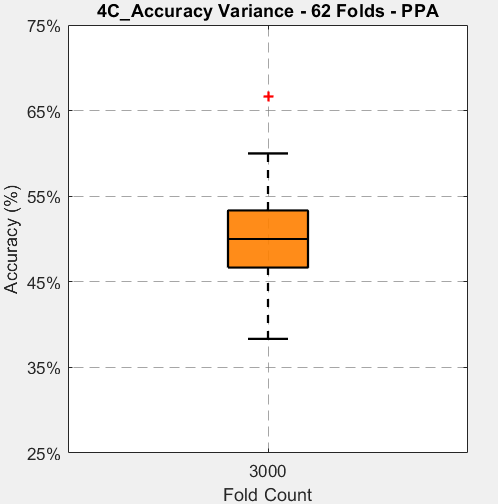
\includegraphics[width = 0.9\textwidth, height = 5cm]{assets/images/box_4C_62_ppa.png}
		\caption{Accuracy Variance Across the Optimal 62 Folds for \gls{4C} Data.}
		\label{fig:4C_62_ppa}
	\end{subfigure}
	\caption[Accuracies At Optimal Fold Count Boxplots For The PPA]{Boxplots Produced During the 'Practical Fold Count' Analysis in the \gls{PPA}.}
 	\label{fig:fold_ppa}
\end{figure}

The accuracy distributions corresponding to the optimal practical fold counts are displayed in \autoref{fig:fold_ppa}. These distributions mirror those obtained from the 3000-fold count analyses, confirming that the classifier's true accuracy can be attained at lower, more  practical fold counts as well.

\subsection{Subject Count \textit{(PPA)} - Results}

In the \gls{2C} analysis (see \autoref{fig:count_2C_ppa}), the classifier begins to perform consistently at around 60\% accuracy once more than 6 subjects are included, gradually increasing to 66.8\% at 15 subjects and then contnueing to oscillate around the final value of 66.4\%. At lower subject counts, performance improves rapidly in a linear fashion as more subjects are added, with the only anomaly occurring at 5 subjects, where a notably precise accuracy of 67.5\% is achieved. This subject count could be leveraged for extremely fast, efficient, and relatively accurate analyses, requiring manipulation of just 20 patterns in total.

\begin{figure}[htbp]
 	\centering
	\begin{subfigure}{0.49\textwidth}
		\centering
		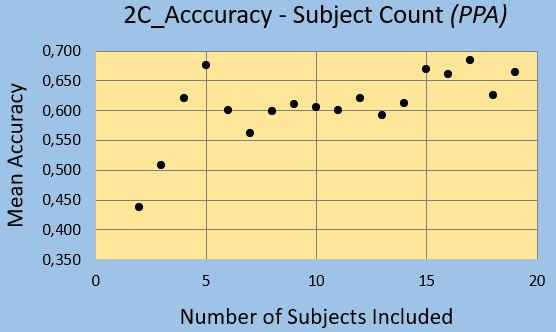
\includegraphics[width = 0.9\textwidth, height = 5cm]{assets/images/subj_count_2C_ppa.png}
		\caption{Accuracy Variance Across Different Subject Counts for \gls{2C} Data.}
		\label{fig:count_2C_ppa}
	\end{subfigure}
	\hfill
	\begin{subfigure}{0.49\textwidth}
		\centering
	 	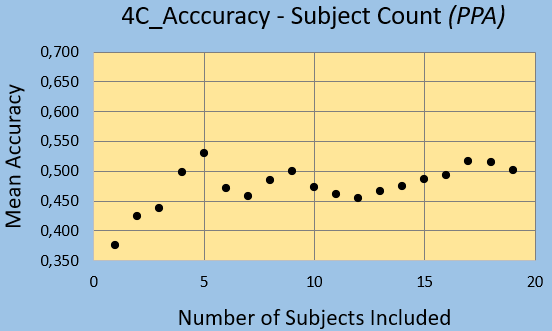
\includegraphics[width = 0.9\textwidth, height = 5cm]{assets/images/subj_count_4C_ppa.png}
		\caption{Accuracy Variance Across Different Subject Counts for \gls{4C} Data.}
		\label{fig:count_4C_ppa}
	\end{subfigure}
	\caption[Accuracies Across Subject Counts For The PPA]{Data Produced During the 'Subject Count' Analysis in the \gls{PPA}.}
 	\label{fig:count_ppa}
\end{figure} 

A similar pattern is observed in \gls{4C} data (see \autoref{fig:count_4C_ppa}), though in an even more stable manner, with smaller deviations from the mean. The same irregularity at 5 subjects is evident, where accuracy peaks at 52.9\%. Stabilization initially occurs around a low point of 47\% until 14 subjects, after which accuracy slightly oscillates around the final accuracy of 50.1\%.

For \gls{MVPA} in the \gls{PPA}, classifier performance follows a more typical pattern, improving as the number of subjects and data points increases. Performance appears to plateau after about 15 subjects, with the potential for even higher accuracy as more data is included. This can be attributed to the consistent magnitude of brain activation in the \gls{PPA} (as shown in \autoref{fig:upa_ppa}), where the signal for places is significantly higher than for other stimuli. This difference becomes more pronounced with the inclusion of additional subjects and data points, enhancing the classifier's ability to distinguish and accurately classify place-related signals. This effect is even more pronounced in the \gls{4C} case, where the disparity between places and other stimuli categories is greater, leading to fewer fluctuations and a more predictable improvement in the classifier's success rate with added data.




%%% End of PPA %%%




\section{Classification Ideal Parameters}

Below is a summary of the variable sets used by the classifier across different functions.

\subsection{Classifier Maximum Accuracy - Results}

The highest classifier performance, 70\%, was achieved in the \gls{2C} analysis for the \gls{FFA}, using 3000 folds and 19 subjects, with a completion time of 114.1\si{second}. Similarly, with the maximum values of 3000 folds and 19 subjects, the \gls{2C} analysis in the \gls{PPA} achieved a 66.4\% success rate in 117.6\si{second}.

Interestingly, the maximum accuracy was not obtained with the largest datasets but rather from the analysis that combined 2-Back and 0-Back signals for each stimulus category.

\subsection{Classifier Maximum Efficiency - Results}

In the \gls{FFA} \gls{2C} analysis with only 4 subjects and the maximum possible 28 folds, the process completes in just 1.2\si{second}, achieving an accuracy of 78.1\%. As for the \gls{PPA}, in the \gls{2C} analysis using 5 subjects and 45 folds, the classifier reaches a success rate of 67.5\% in just 1.4\si{second}.

While these results cannot be broadly generated with larger datasets, they provide valuable insight into the classifier's potential performance when the data is meticulously screened for artifacts and signals from different stimulus categories are distinctly robust.

\subsection{Classifier Maximum Practicality - Results}

In terms of combining efficiency, precision, and reliability, the \gls{2C} analysis with 11 subjects and 69 folds achieves 70\% accuracy in just 2.6\si{second} for the \gls{FFA}. This matches the success rate of the exhaustive 3000-fold analysis but accomplishes it in a fraction of the time, while also being based on a sufficiently large dataset to ensure reproducible results. In the \gls{PPA}, analyzing \gls{2C} data from 15 subjects at 49 folds yields a classifier accuracy of 66.8\% in 2.9\si{second}. The success pattern is similar to that observed for the \gls{FFA}, although in this case, the data reduction compared to the maximum accuracy analysis was less severe.

These settings should form the basis for the bulk of the analyses, as increasing the magnitude of variables would only demand more computational power and time without offering significant additional benefits.
\pagebreak
\chapter{Conclusions}
\label{sec:conclusions}

Significant progress has been made in brain functional mapping over the past few decades. This thesis has shown the feasibility and efficiency of using \gls{MVPA} in both the \gls{FFA} and \gls{PPA} to decode category-specific neural patterns. As more discoveries link specific brain functions to distinct regions, the methodology presented here offers a framework that can be adapted to a wide range of research questions, both within and beyond the realm of visual processing. The thorough analysis of baseline signals, which integrates traditional univariate methods with advanced multivariate techniques, sets a standard for future research. It also lays the groundwork for the development of more sophisticated tools, enhancing both the quality of results and the efficiency of resource use in the development process.

This research also offers practical implications for the development of more efficient and reliable brain-computer interfaces \gls{BCI}s. The findings demonstrate that accurate neural decoding can be achieved with a reduced number of folds and subjects, significantly lowering the computational cost and time required. This is particularly relevant for clinical applications, where quick and accurate neural decoding could enhance the effectiveness of neurofeedback and other therapeutic interventions.

Looking ahead, future research should explore several avenues to build upon and refine the findings of this study. First, utilizing data from large-scale functional mapping projects, similar in scope to the \gls{HCP}, could significantly enhance the generalizability, reliability, and statistical power of the results. Additionally, longitudinal studies would be valuable in examining how neural representations evolve over time or with training, offering insights into the plasticity of neural coding. 

Another promising direction is to apply \gls{MVPA} to other brain regions involved in visual processing, such as the \gls{OFA} and the \gls{LOC}. Expanding the analysis to these areas could provide a more comprehensive understanding of the neural mechanisms underlying face and place recognition, potentially revealing the hierarchical processing stages across different cortical regions.

Lastly, integrating \gls{MVPA} with other neuroimaging techniques like \gls{EEG} or \gls{MEG} could shed light on the temporal dynamics of category-specific processing. This multimodal approach would bridge the gap between the high spatial resolution of \gls{fMRI} and the superior temporal resolution of \gls{EEG}/\gls{MEG}, offering a more complete and nuanced picture of neural processing.

Despite the promising results, this study is not without its limitations. A notable constraint is the relatively small sample size, which may impact the statistical power and generalizability of the findings. Additionally, the study primarily focused on two specific brain regions, the \gls{FFA} and \gls{PPA}. While these areas are key to face and place recognition, and were chosen due to the strong established connections between them and their associated functions, other relevant brain areas were not explored. This narrow focus could limit the broader applicability of the \gls{MVPA} techniques and the generalization of these classification methods to more complex cognitive processes.

Finally, the study's reliance on data from the \gls{HCP} may introduce some bias, as this dataset is preprocessed and may not fully represent the variability and complexity of raw \gls{fMRI} data. Future studies should aim to validate these findings using raw, unprocessed data to ensure the robustness of the conclusions.

In conclusion, this thesis not only advances our understanding of the neural mechanisms underlying category-specific visual processing but also lays the groundwork for future research that could lead to significant developments in both theoretical and applied neuroscience.

% Print the glossary entries
\pagebreak
\printglossaries

% Print the references
\pagebreak
\printbibliography[heading=bibintoc]

%\appendix
%\input{Appendices/algorithms.tex}
%\input{Appendices/snippets.tex}
%\input{Appendices/code.tex}

\end{document}

% Optioal commands to add below

% If you use the \maketitle command to have an extra page after the cover with just tile and author.
%\title{\mytitle}
%\author{Nikolaos Kasapakis}
%\date{}

% Highlighting yaml code in listings.
% https://tex.stackexchange.com/questions/152829/how-can-i-highlight-yaml-code-in-a-pretty-way-with-listings
% \newcommand\YAMLcolonstyle{\color{red}\ttfamily\footnotesize}
% \newcommand\YAMLkeystyle{\color{black}\ttfamily\bf\footnotesize}
% \newcommand\YAMLvaluestyle{\color{blue}\ttfamily\footnotesize}
